
\documentclass[12pt,english]{article}
\usepackage{mathptmx}
\renewcommand{\familydefault}{\rmdefault}
\usepackage[T1]{fontenc}
%\usepackage[utf8]{luainputenc}
\usepackage[letterpaper]{geometry}
\geometry{verbose,tmargin=3cm,bmargin=2cm,lmargin=25mm,rmargin=25mm}
\usepackage{color}
\usepackage{babel}
\usepackage{footnote}
\addto\shorthandsspanish{\spanishdeactivate{~<>}}

\usepackage{array}
\usepackage{longtable}
\usepackage{rotating}
\usepackage{float}
\usepackage{rotfloat}
\usepackage{multirow}
\usepackage{amssymb}
\usepackage{graphicx}
\usepackage{setspace}
\usepackage{nomencl}

%Packages of mindmap

\usepackage[utf8]{inputenc}
%\usepackage{dtklogos}
\usepackage{tikz}
\usetikzlibrary{mindmap,shadows}
% Information boxes
\newcommand*{\info}[4][16.3]{%
  \node [ annotation, #3, scale=0.65, text width = #1em,
          inner sep = 2mm ] at (#2) {%
  \list{$\bullet$}{\topsep=0pt\itemsep=0pt\parsep=0pt
    \parskip=0pt\labelwidth=8pt\leftmargin=8pt
    \itemindent=0pt\labelsep=2pt}%
    #4
  \endlist
  };
}

% the following is useful when we have the old nomencl.sty package
\providecommand{\printnomenclature}{\printglossary}
\providecommand{\makenomenclature}{\makeglossary}
\makenomenclature
\onehalfspacing
\usepackage{hyperref}
\hypersetup{
    colorlinks = true,
    allcolors = blue,    
}
\makeatletter

%%%%%%%%%%%%%%%%%%%%%%%%%%%%%% LyX specific LaTeX commands.
\DeclareRobustCommand*{\lyxarrow}{%
\@ifstar
{\leavevmode\,$\triangleleft$\,\allowbreak}
{\leavevmode\,$\triangleright$\,\allowbreak}}
%% Because html converters don't know tabularnewline
\providecommand{\tabularnewline}{\\}

%%%%%%%%%%%%%%%%%%%%%%%%%%%%%% Textclass specific LaTeX commands.
\newenvironment{lyxlist}[1]
{\begin{list}{}
{\settowidth{\labelwidth}{#1}
 \setlength{\leftmargin}{\labelwidth}
 \addtolength{\leftmargin}{\labelsep}
 \renewcommand{\makelabel}[1]{##1\hfil}}}
{\end{list}}

%%%%%%%%%%%%%%%%%%%%%%%%%%%%%% User specified LaTeX commands.
\usepackage{lscape}
\addto\captionsspanish{
\def\tablename{Tabla}
\def\listtablename{\'Indice de tablas}
}

\makeatother

\begin{document}

\title{PASSIVE DYNAMIC SYSTEM FOR ENERGY RETURNING ON TRANSTIBIAL PROSTHESES}
\maketitle
\begin{center}
 \textbf{{\large DAAD CALL FOR RESEARCH PROPOSALS}}
\par\end{center}

\begin{center}
RESEARCH PROPOSAL 
\par\end{center}

\begin{description}
\item [{NAME:}] \author{Edwin Nikolay Prieto Parrado} \textbf{ID:}C.C 1071162895.
\item [{DEGREE:}] B.E. in Mechatronics - Universidad de San Buenaventura \\ M.Sc. in Mechatronical Engineering - Universidad Militar Nueva Granada.
\item[{POSITION: }] PhD Student of Mechanics and Mechatronics School at Universidad Nacional de Colombia (UNAL) \\ Student Auxiliary Professor at UNAL.
\item[{DATE OF BIRTH: }] February 17th 1987.
\item[{NATIONALITY: }] Colombian
\item[{HOME ADDRESS: }] 12th St. 3rd. Av. -05 - La Calera, Cundinamarca, Colombia.
\item[{WORK ADDRESS: }] 45th Av. 26th St -85 - Edificio Uriel Gutiérrez
Bogotá D.C.,  Colombia.
\item[{PHONE NUMBER: }] +57 (1) 3003501177 - +57 (1) 8600428.
\item[{E-mail: }] \href{mailto:enprietop@unal.edu.co}{  enprietop@unal.edu.co}
\item[{TITLE: }]\emph{{\large PASSIVE DYNAMIC SYSTEM FOR ENERGY RETURNING ON TRANSTIBIAL PROSTHESES}}


\item [{SUPERVISOR:}] Prof. Dr-Ing. Carlos Julio Cortés
Rodríguez.
\item [{CO-SUPERVISOR:}] Eng. Andrés Tovar PhD.

 \textbf{FIELD OF STUDY:} Computational Modeling, Multibody Rigid and Flexible Dynamics, Lower Limb Prosthesis, Gait Analysis, Biomechanics, Cellular solids.

\textbf{KEYWORDS:} Passive Actuators, Cellular solids, Prosthesis, Ankle joint biomechanics.


\end{description}
\newpage
\renewcommand*\contentsname{Summary}
\tableofcontents
\newpage


\section{MOTIVATION}

The demand of Lower Limb Prosthesis (LLP) is higher every day around the world, due to the constant increment of principal causes of amputations. Ziegler \emph{et al.}\cite{Ziegler-Graham2008} showed that in United States of America amputations at 2008 were caused by Vascular disease (including diabetes) with 53,95\% of the total of amputees, followed by trauma (e.g. accidents, warfare, among others) with 44,90\%, and finally cancer with 1,15\%. They estimate that in 2050 the number of amputees will have risen to 3,6 millions \cite{Ziegler-Graham2008}. 

Recently, the \emph{International Diabetes Federation (IDF\nomenclature{IDF}{International Diabetes Federation})
} in 2015 published the IDF atlas, which has announced that the number of people with diebetes is between 340-536 millions \cite{IDF2015}. Moreover, They estimate this sickness will have affected to 642 million of people worldwide.
  
In addition, diabetes affects mostly the lower limbs, having potential risks to suffer peripheral arterial illness, diabetic foot and as a result, an amputation. The possibility of suffering an amputation will depend on race, gender, and age of the population, being different on many countries. Below, It is showed the number of amputations per 100.000 habitants caused by diebetes according to Kroger and Knut \cite{KrogerKnut2015}. 
En consecuencia de lo anterior, la diabetes afecta en su mayoría a
los \emph{miembros inferiores (MMII\nomenclature{MMII}{Miembro(s) Inferior(es)}),
}generando enfermedades arteriales periféricas, síndrome de pie diabético
y posteriormente su amputación. El riesgo de generar amputación a
causa de esta enfermedad dependerá de la edad, sexo y raza de la población,
siendo diferente el número de amputaciones por país. En la Fig. \ref{fig:N=0000FAmero-de-amputaciones}
se muestra la cantidad de amputaciones en MMII por cada cien mil habitantes
en determinadas naciones que cuentan con esa estadística 

\begin{figure}[H]
\begin{centering}
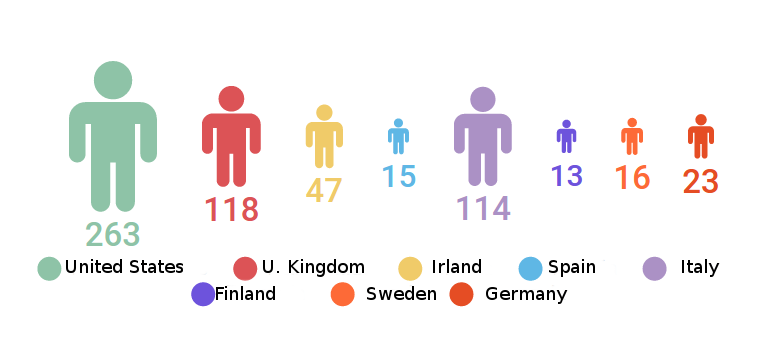
\includegraphics[scale=0.5]{ampperyear}
\par\end{centering}

\caption{\label{fig:N=0000FAmero-de-amputaciones}Número de amputaciones de
MMII por cada 100.000 habitantes durante un rango de tiempo determinado
individualmente por nación. Adaptado de Kroger \cite{KrogerKnut2015}. }


\end{figure}


Ahora bien, del panorama nacional, se estima que la primera causa
de amputación de MMII es la diabetes y no el conflicto armado. Aunque
no existan cifras oficiales de amputación por esta patología en nuestro
país, en el estudio de Ramírez \cite{Ramirez2014} se dedujo qué:
al existir aproximadamente 1.7 millones de diabéticos en Colombia,
y paralelamente sus estadísticas reflejan que el 15\% de la población
diabética a nivel mundial desarrolla una úlcera de pie, la cual es
precedente del 85\% de las amputaciones de extremidades inferiores,
da como resultado un panorama mayor a 200.000 amputados de MMII en
el país. De otra parte, Pinilla \emph{et al.} \cite{Pinilla2011}
determinó que el 1.6\% de 307 pacientes Colombianos sufrió algún tipo
de amputación a causa de la diabetes, y de esa población el 76.2\%
mencionó que no les fue revisada la afectación anteriormente,  sabiendo
que el 78.2\% no recibió educación sobre el cuidado del pie con diabetes
mellitus tipo II.

De otra parte, el conflicto armado también contribuye al incremento
de amputaciones en el mundo, durante la segunda guerra mundial se
registraron 14.912 víctimas con amputación sólo en Estados Unidos,
mientras que en la guerra de Vietnam se generaron aproximadamente
5.238 amputaciones \cite{Laferrier2010a}. Actualmente, la guerra
de Irak y Afganistán contra EE.UU. dejó un balance de 913 amputados
a julio de 2009, de los cuales 723 fueron amputados de miembro inferior\cite{Fergason2010}. 

De igual modo, otro país que presenta gran cantidad de afectados por
el conflicto armado es Colombia, de acuerdo al estudio realizado por
el DAICMA\footnote{Dirección para la Acción Integral contra Minas Antipersonal}
(con corte a marzo de 2016 \cite{PAICMA}), del panorama nacional
se encuentran aproximadamente 11.405 víctimas (entre civiles y militares)
a causa de las MAP (Minas Antipersonal), MUSE (Munición sin Explotar)
y AEI (Artefactos Explosivos Improvisados). A su vez, de acuerdo a
un reporte de la Industria Militar de Colombia \cite{Prieto2014}
del 90\% de esas víctimas son amputados de MMII. De la información
suministrada desde 2009 hasta marzo de 2014, se encontró que el consumo
nacional anual de prótesis de pie del total de víctimas por el conflicto
fue de 691 prótesis aproximadamente, mientras que el consumo de prótesis
de rodilla osciló las 188 unidades.

Aunque comercialmente las prótesis de MMII superan la demanda de prótesis
para miembros superiores en gran proporción, las investigaciones son
equilibradas. De acuerdo a Eshraghi \emph{et al.}\cite{Eshraghi2013}
el 53\% de las cien investigaciones en protésica con mayor número
de citaciones indexadas, llevadas a cabo desde 1981 hasta 2013, se
han centrado en los miembros inferiores, mientras que el 41\% han
sido dirigidas a los miembros superiores y el 6\% restante a temas
generales en prótesis. Del porcentaje de investigaciones en MMII,
se presenta la Fig. \ref{fig:Porcentaje-de-investigaci=0000F3n} que
muestra las tendencias en investigación de este miembro en específico.

\begin{figure}
\begin{centering}
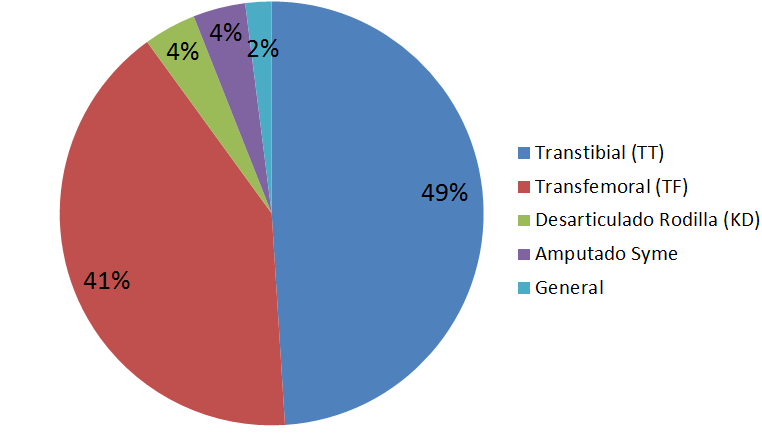
\includegraphics[scale=0.45]{estapies}
\par\end{centering}

\caption{\label{fig:Porcentaje-de-investigaci=0000F3n}Porcentaje de investigación
en temas específicos con los miembros inferiores. Tomado y traducido
de \cite{Eshraghi2013}. }
\end{figure}


Lo anterior es indicio de que las investigaciones y desarrollos en
protésica siguen en continuo desarrollo, dado que la remoción del
miembro genera diversos inconvenientes en la marcha del afectado -que
a la fecha- no han sido subsanados. Las implicaciones fisiológicas
sobre la amputación generan alteraciones en la marcha, lo que a futuro
causará otras patologías no asociadas a la amputación directamente
\cite{Lemoyne}. En la sección \nameref{sub:Estado-del-conocimiento:}
se detallan estas alteraciones dependiendo del tipo de prótesis implementada.

Otro aspecto importante es la capacidad económica de las poblaciones
en desarrollo, lo que permite adquirir dispositivos protésicos de avanzada tecnología. Por otra parte, para los países subdesarrollados, se sacrifica bienestar adquiriendo dispositivos de bajo grado de movilidad y de menor tecnología para una población activa en su mayoría \cite{Lemoyne}.

Por lo anterior, es de gran importancia seguir contribuyendo al desarrollo
de dispositivos protésicos que brinden una mejor calidad de vida a los amputados de MMII mejorando las alteraciones presentes en la marcha, lo anterior se podría lograr a través del mejoramiento de la eficiencia energética de las prótesis sin necesidad de recurrir a actuadores que requieran fuentes de energía externa. Se estima que al no incurrir en este tipo de actuadores, el costo final de producción podría ser inferior a una prótesis activa.


\section{GENERALIDADES}

\printnomenclature{}


\subsection*{Conceptos Generales}
\begin{description}
\item [{Prótesis}] \textbf{pasivas de pie:} A estas prótesis se les denomina
pasivas cuando no hay algún tipo de contribución energética mecánica
externa. Estas prótesis se dividen en dos categorías: i) prótesis
convencional: en donde la prótesis cumple una función netamente estética
y ii) prótesis funcionales (en donde están inmersas las prótesis de
Almacenamiento de Energía y Retorno (ESR por sus siglas en inglés\nomenclature{ESR}{\emph{Energy Storage and Return} / Almacenamiento de Energía y Retorno}))
cuyo propósito es restablecer alguna función del pie y tobillo \cite{Versluys2009}.
\item [{Prótesis}] \textbf{activas de pie: }En estas hay una contribución
de energía mecánica externa bien sea en la fase de balanceo (B) o
en la fase de apoyo. En la literatura anglosajona son conocidas como
\emph{Bionic Prostheses} ó \emph{Powered prostheses} \cite{Cherelle2014a}.
\item [{Trabajo}] \textbf{neto: }Cuando se habla de trabajo neto, específicamente
se refiere al trabajo cíclico que realiza algún sistema músculo-tendinoso,
el cual se obtiene a partir de la integral de linea de los parámetros
de fuerza vs. longitud muscular (ver Fig. \ref{fig:Ciclo-de-trabajo}),
también se puede calcular mediante la obtención de la potencia instantánea
del músculo. A manera de ejemplo, cuando el músculo se contrae y se
le aplica una fuerza a tensión, se dice que está realizando un trabajo
positivo por parte de ese miembro. Por otro lado, si el músculo se
extiende y se aplica nuevamente fuerza a tensión, se dice que el trabajo
es negativo \cite{Altringham1990}. 


\begin{figure}
\centering{}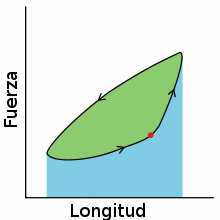
\includegraphics[scale=0.5]{workloop}\caption{\label{fig:Ciclo-de-trabajo}Ciclo de trabajo muscular. Las flechas
indican la trayectoria temporal del ciclo de trabajo. La zona verde
indica el trabajo neto, la zona azul indica el trabajo perdido. La
suma de las dos zonas indica el trabajo total. Adaptado de Wikipedia Inc. \cite{workloop}}.
\end{figure}


\item [{Trabajo}] \textbf{mecánico en la marcha humana: }Éste se divide
en dos tipos de trabajo, el primero es el trabajo interno, el cual
está asociado con el movimiento de los miembros en relación al \emph{Centro
de Masa (COM\nomenclature{COM}{\emph{Center of Mass} / Centro de Masa}) }corporal
sobre el plano sagital. En cambio, el trabajo externo es el realizado
por las fuerzas externas cuyo comportamiento se plantea en la Fig.
\ref{fig:Modelo-biomec=0000E1nico-de} y el cual se puede estimar
a partir de la medición de la \emph{fuerza de reacción al piso (GRF\nomenclature{GRF}{\emph{Ground Reaction Forces} / Fuerzas de Reacción al Piso})}
.


\begin{figure}
\begin{centering}
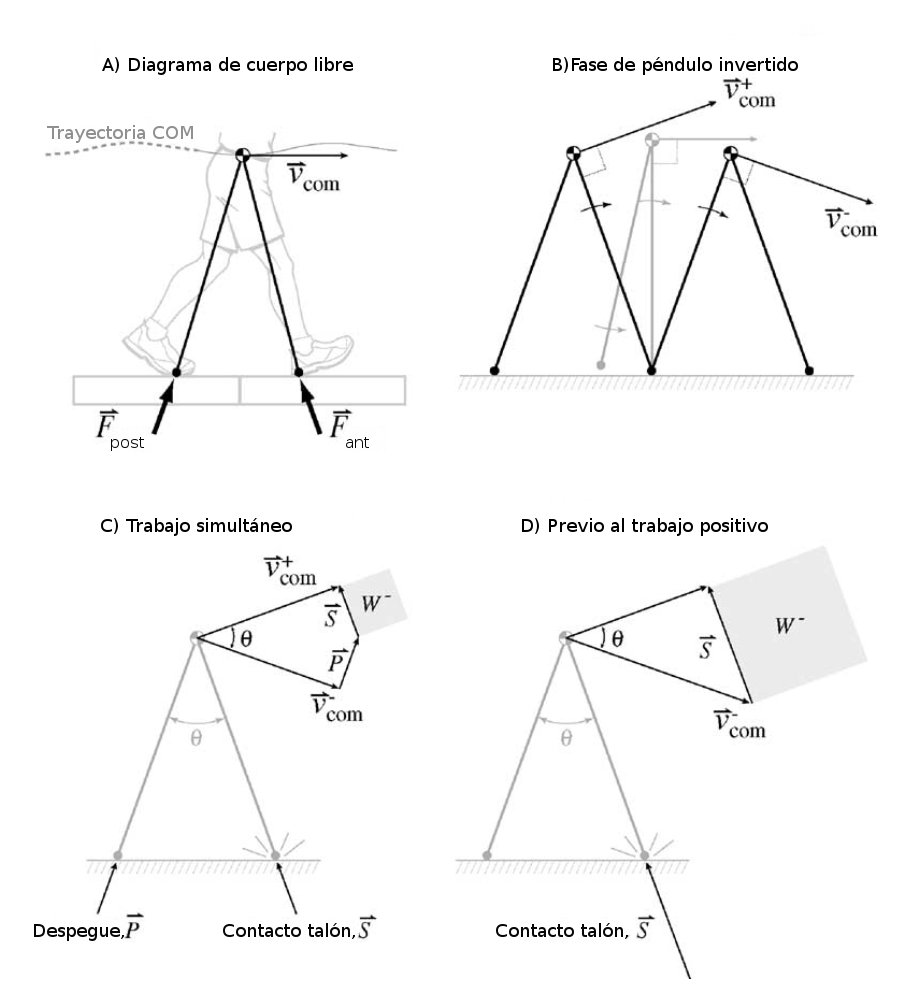
\includegraphics[scale=0.45]{workLL}
\par\end{centering}

\caption{\label{fig:Modelo-biomec=0000E1nico-de}Modelo biomecánico de marcha
de Kuo, en el cual se representa el trabajo individual de cada miembro
(anterior y posterior) en la marcha bípeda durante el apoyo doble.
En A) se muestra la velocidad del COM ($\protect\overrightarrow{v_{COM}}$)
y las fuerzas de reacción de los miembros posteriores ($F_{post}$)
y anteriores ($F_{ant}$). En B) la velocidad del COM es perpendicular
al miembro en fase de apoyo, los signos denotan los límites superior
e inferior respectivamente. En C) se representa la transición paso
a paso la cual requiere de un direccionamiento de la velocidad del
COM, $P$ y $S$ representan impulsos escalones que emulan las GRF.
Por último, en D) se visualiza la magnitud del trabajo negativo externo
realizado por el miembro anterior previo a la generación de trabajo
positivo del miembro posterior. Tomado y traducido de \cite{Donelan2002}.}
\end{figure}



Ahora bien, para estimar el trabajo interno se debe calcular la dinámica
inversa de la marcha a través de modelos biomecánicos computacionales
o mediante el software del laboratorio de marcha.

\item [{Costo}] \textbf{metabólico:} Es la cantidad de energía consumida
como resultado de la realización de una actividad que demande trabajo,
usualmente se expresa en calorías. Su medición se realiza mediante
la calorimetría indirecta, la cual mide volumen de oxígeno neto ($\dot{V}O_{2}$),
frecuencia cardíaca y tasa de intercambio respiratorio (cuyo valor
usualmente es 1.0). El $\dot{V}O_{2}$ se puede convertir a Julios
usando la equivalencia energética de 20.1 $J$ por $ml*O_{2}$ \cite{Mian2006}.
El costo metabólico se obtiene de la división del gasto energético
($\frac{J}{kg*min}$) por la velocidad ($m/min$).
\item [{Transición}] \textbf{paso a paso: }En el estudio del modelo biomecánico
de Donelan \emph{et al.} \cite{Donelan2002a} se concluye que la fase
de balanceo conserva la energía mecánica y por tanto no requiere trabajo
para rotar alrededor de su COM, sin embargo la transición de los miembros
en el apoyo doble si requiere trabajo, por tanto será el mayor determinante
en el costo metabólico de la marcha y es en la transición paso a paso
donde se determina esta variable.
\item [{Fase}] \textbf{de marcha enfocada a la amputación transtibial:}
El ciclo de marcha se define como el intervalo de tiempo entre dos
sucesos repetitivos en la marcha, generalmente se define el ciclo
desde el \emph{Contacto Inicial (CI\nomenclature{CI}{Contacto Inicial})}
del pie derecho hasta que se repita el mismo suceso. El pie izquierdo
repetirá el mismo ciclo pero desfasado.



\begin{figure}
\begin{centering}
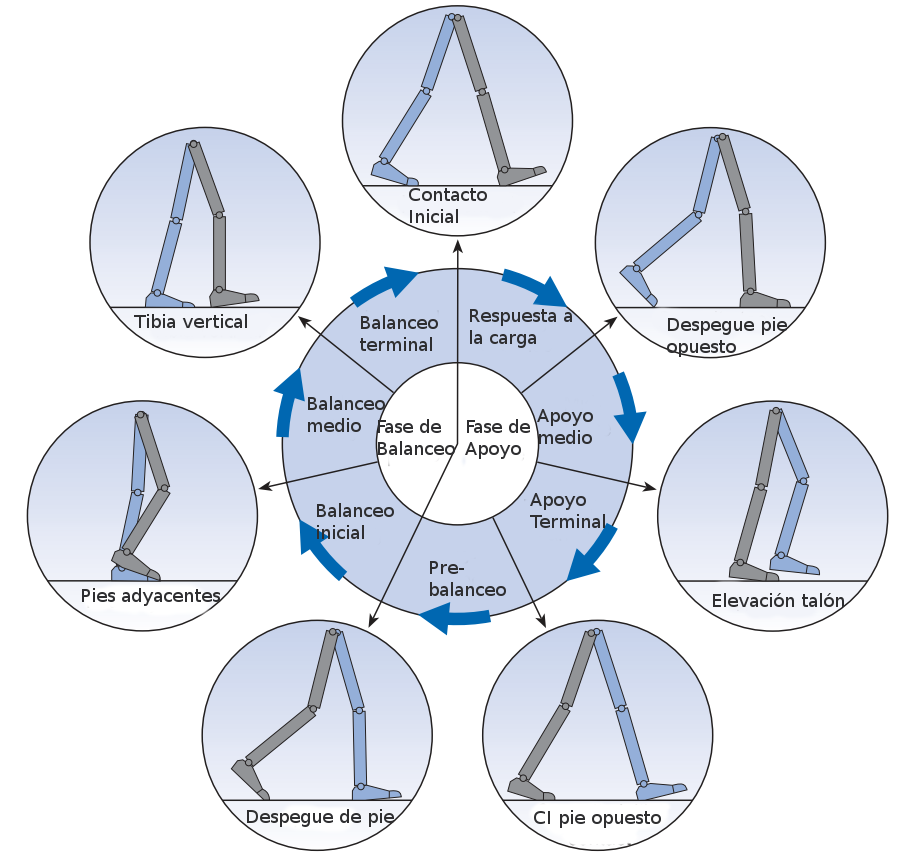
\includegraphics[scale=0.33]{Singlephaseesp.png}
\par\end{centering}


\label{fig:Posici=0000F3n-de-los}Posición de los miembros inferiores
durante un ciclo de marcha estándar enfocado al pie derecho. Adaptado
y traducido de Whittle\cite{Whittle2007}.

\end{figure}



En la Fig. \ref{fig:Posici=0000F3n-de-los} se muestra el ciclo de
marcha completo distribuido en porcentajes temporales sobre el ciclo
completo, el cual se divide de la siguiente manera:


\begin{table}[H]
\caption{Distribución temporal de la marcha. Tomado y traducido de \cite{Lemoyne} }


\centering{}%
\begin{tabular}{|c|c|c|c|}
\hline 
\multicolumn{2}{|c|}{Fase de marcha} & \multicolumn{2}{c|}{Porcentaje de fase de marcha}\tabularnewline
\hline 
\hline 
\multirow{3}{*}{Fase de apoyo} & Doble apoyo inicial & 10\% & \multirow{3}{*}{60\%}\tabularnewline
\cline{2-3} 
 & Apoyo simple & 40\% & \tabularnewline
\cline{2-3} 
 & Doble apoyo terminal & 10\% & \tabularnewline
\hline 
Fase de balanceo & Inicial - Media - Terminal & 40\% & 40\%\tabularnewline
\hline 
\end{tabular}
\end{table}



Ahora, enfocándose específicamente en la dinámica de la articulación
tibio-astragalina, se presenta la fisiología de esta junta desde el
punto de vista del trabajo mecánico interno a realizar por esta articulación
(Ver Fig.\ref{fig:Gr=0000E1fica-de-torque}).


\begin{figure}[H]
\begin{centering}
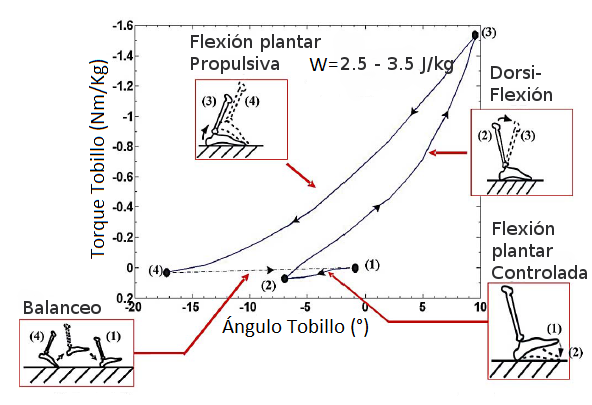
\includegraphics[scale=0.7]{cinneticatobillo}
\par\end{centering}

\caption{\label{fig:Gr=0000E1fica-de-torque}Gráfica de torque vs. ángulo de
la articulación del tobillo a una velocidad de 1.25 m/s. El segmento
(1-2) representa el Contacto Plantar (\nomenclature{CP}{Contacto Plantar en flexión}CP)
en flexión, el (2-3) representa la dorsiflexión controlada (\nomenclature{DC}{Dorsiflexión Controlada}DC)
y el (3-4) representa la \emph{Propulsión Plantar (\nomenclature{PP}{Propulsión Plantar}PP)}.
La línea punteada (4-1) muestra la \emph{fase de balanceo del pie
(\nomenclature{B}{Fase Balanceo}B)}. \nomenclature{W}{Trabajo}W
es el \emph{trabajo mecánico interno} generado. Adaptado y traducido
de \cite{Au2009}}
\end{figure}


\item [{Dinámica}] \textbf{pasiva:} Se refiere al comportamiento dinámico
de actuadores, robots u organismos sin necesidad de requerir energía
de una fuente externa (e.g., baterías, combustibles, etc) para su
funcionamiento. Los dispositivos que no requieren fuentes de potencia
externa son considerados pasivos y su comportamiento se denomina usualmente
como ``dinámica pasiva'' \cite{Wisse2006}. 
\item [{Actuador}] \textbf{rígido:} De acuerdo a Cherelle \emph{et al.}
\cite{Cherelle2014a} un actuador rígido es aquel que no posee la
capacidad de almacenar energía por deformación elástica (i.e., motor
eléctrico).
\item [{Actuador no rígido (\it{compliant actuator}):}] Es lo
apuesto a una actuación rígida, ésta es capaz de almacenar energía
potencial por deformación elástica \cite{Cherelle2014a}.
\item [{Cuasi-rigidez:}] Es un término para definir la rigidez dinámica
de las extremidades inferiores (e.g., tobillo, rodilla y cadera),
la cuasi-rigidez es definida globalmente como la tangente del mejor
ajuste lineal de la gráfica torque-ángulo (Ver Fig. \ref{fig:Cuasi-rigidez-de-la}) de una articulación sobre el ciclo de marcha o sobre una porción de la fase de apoyo \cite{Shamaei2013}
. En el estudio de Rouse
\emph{et al.} \cite{Rouse2013a} se diferenció este concepto frente
a los dispositivos pasivos y activos. En el primero, el concepto sigue
siendo el mismo que el anterior, pero en el segundo, es el equivalente
al control aplicado para obtener la trayectoria de la rigidez del
actuador (e.g. control del torque y velocidad del motor).


\begin{figure}
\begin{centering}
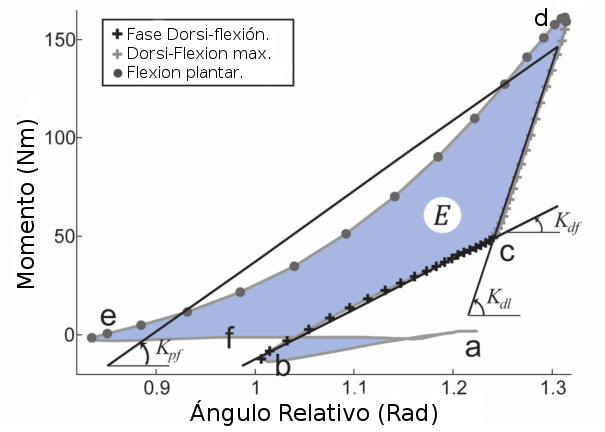
\includegraphics[scale=0.5]{quasirigidez}
\par\end{centering}

\caption{\label{fig:Cuasi-rigidez-de-la}Cuasi-rigidez de la articulación de
tobillo a velocidad constante de 1.75 m/s. Las letras a-f corresponden
a las diferentes instancias de la fase de marcha como son: a) CI;
b) Apoyo Medio; c y d representan la DC inicial y terminal respectivamente;
e) Despegue de pie; f) fase de B. La cuasi-rigidez es calculada basándose
en el mejor ajuste lineal de los puntos b-c para la DC inicial ($K_{df}$),
c-d para la DC terminal ($K_{dl}$) y d-e para la descarga en la PP
($K_{pf}$). ($E$) representa el trabajo positivo realizado en la
articulación. Adaptado de Shamaei \emph{et al.} \cite{Shamaei2013}.}
\end{figure}



El mejor ajuste lineal de cada instancia mostrada en la Fig. \ref{fig:Cuasi-rigidez-de-la} se determinó mediante una regresión de mínimos cuadrados por Shamaei \emph{et al.} \cite{Shamaei2013} de la siguiente manera:


\begin{equation}
K_{pf}\thickapprox 11+\frac{34.6WH-3.81WHV-741}{\theta_{df}} \label{eq:1}
\end{equation}



\begin{equation}
K_{dl}\thickapprox \frac{-1596-(18.0V^{2}-88.8V+118.9)WHV+146.2W}{\theta_{dl}} \label{eq:2}
\end{equation}



\begin{equation}
K_{pf}\thickapprox 17-\frac{(3.68V-10.68)WHV^{3}-56.61W}{\theta_{pf}} \label{eq:3}
\end{equation}

\begin{eqnarray}
E &=&15500+(510.8-37.9W+14.25VW)(\theta_{df}+\theta_{dl}) \nonumber \\ && +((39.6-24.4V+3.47HV^{3}-0.84HV^{4})W-803.6)(\theta_{pf}-\theta_{dl})\label{eq:8}
\end{eqnarray}




Dónde $\theta_{df},\theta_{dl},\theta_{pf}$ son los ángulos entre
los puntos $b-c$, $c-d$ y $d-e$ respectivamente (Ver Fig. \ref{fig:Cuasi-rigidez-de-la}),
$W$ es el peso corporal, $V$ es la velocidad preferida del usuario y $H$ es
la altura corporal, $E$ es el trabajo realizado. La calidad de la regresión se da por el $R^{2}$, el cual fue de 75.4\%, 75.3\%, 81.3\% y 80.5\% para las ecuaciones \ref{eq:1},\ref{eq:2}, \ref{eq:3} y \ref{eq:8} respectivamente.

De lo anterior se puede deducir que la cuasi-rigidez depende directamente
de la antropometría y de su velocidad preferida, por tanto una prótesis
para esta articulación podría ser más eficiente si se diseñara de
acuerdo a sus características individuales.
\item[{Dinámica Multi-cuerpo Deformable \cite{Shabana2013}: }] Cuando la distancia entre dos partículas del cuerpo permanecen constantes, se dice que las fuerzas que interactúan provocan una aceleración lineal y angular uniformes a lo largo del curpo, a esto se le conoce como dinámica multi-cuerpo rígida. 
A diferencia de lo anterior, en la dinámica deformable, el movimiento del cuerpo depende de la deformación relativa de una partícula frente a sus partículas vecinas. La cinemática de los cuerpos de bajas deformaciones se puede describir mediante la matriz de gradientes de posición del vector, así:
\begin{equation}
J=\frac{\partial{\xi}}{\partial{\bf{x}}}=\frac{\partial{\xi}}{\partial{\bf{\bar{x}}}}\frac{\partial\bf{\bar{x}}}{\partial{\bf{x}}}=\frac{\partial{\xi}}{\partial{\bf{\bar{x}}}}A^{T}
\end{equation}
En donde el Jacobiano $J$ dependerá de la matriz de desplazamientos $\xi$ del vector y de sus coordenadas generalizadas $\bf{x}$, que a su vez dependerán de la orientación del sistema $\bf{\bar{x}}$, la matriz $A^{T}$ corresponde a la matriz de transformación ortogonal.

De la cinemática surgen los componentes de deformación que para el caso de bajas deformaciones se presenta la siguiente aproximación:
\begin{equation}
\varepsilon_{m}\approx\frac{1}{2}[\bar{J}^{T}+\bar{J}] \label{eq:5}
\end{equation}
En la ecuación \ref{eq:5}, los componentes de la deformación $\varepsilon_{m}$ dependerán del jacobiano del sistema  $\bar{J}$ referente al sistema de coordenadas generalizado.
Ahora bien, para expresar la dinámica de cada cuerpo del sistema, se utilizan las ecuaciones de Lagrange para derivar las ecuaciones diferenciales de movimiento, teniendo como resultado la siguiente expresión:
\begin{equation}
M^{i}\ddot{q}+K^{i}q^{i}+C_{q^{i}}^{T}\lambda=Q_{e}^{i}+Q_{v}^{i},\:i=1,2\ldots n_{b} \label{eq:6}
\end{equation}
Donde $M$ es la matriz de masa de cada cuerpo $i$, las coordenadas generalizadas de cada cuerpo $q$ se derivan para encontrar su aceleración relativa al punto de origen, $K$ representa la matriz de rigidez, $C_{q^{i}}^{T}$ representa las restricciones, $\lambda$ es el vector de los multiplicadores de Lagrange. En el otro lado de la ecuación se tiene que $Q_{v}^{i}$ es el vector de velocidad cuadrática resultado de la diferenciación de la energía cinética con respecto al tiempo y a las coordenadas del cuerpo, finalmente $Q_{e}^{i}$ representa el vector de fuerzas generalizadas.



\end{description}

\section*{\label{sub:Estado-del-conocimiento:}ESTADO DEL CONOCIMIENTO}


\subsection*{Estado actual de la protésica transtibial:}

La justificación indica la tendencia mundial de continuar investigando
las patologías de la amputación transtibial, debido a la complejidad
de la articulación de tobillo y de la demanda energética por parte
del usuario. Grandes avances en la protésica de miembro inferior se
han realizado para mejorar la naturalidad en la marcha, bien sea en
prótesis pasivas con respuesta elástica (ESR), las cuales
en el mercado se pueden encontrar un sinfín de productos con características
diversas, o en prótesis activas (conocidas también como prótesis
biónicas), las cuales han mostrado una mejoría con respecto a las
pasivas en términos biomecánicos y fisiológicos. El estado actual
de los dispositivos protésicos de pie pasivos se listan en el artículo
de Versluys \emph{et al.} \cite{Versluys2009} y la clasificación
de prótesis hasta las activas se enuncian en la revisión de Cherelle
\emph{et al.} \cite{Cherelle2014a}, las cuales se muestran en la
Fig. \ref{fig:Categorizaci=0000F3n-seg=0000FAn-Cherelle}.

\begin{figure}[H]
\begin{centering}
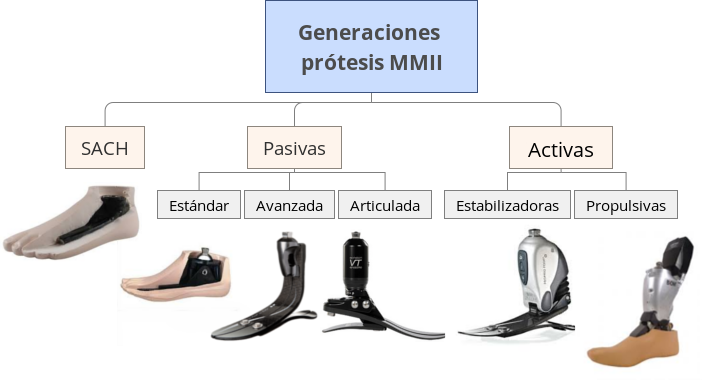
\includegraphics[scale=0.68]{Generacionesprotesis}
\par\end{centering}

\caption{\label{fig:Categorizaci=0000F3n-seg=0000FAn-Cherelle}Categorización
según Cherelle \emph{et al.}\cite{Cherelle2014a} de las prótesis
comerciales. De izquierda a derecha: el pie SACH, el pie de eje sagital,
pie OSSUR$\circledR$ flex foot, Echelon foot$\circledR$, pie Proprio
de OSSUR$\circledR$ y por último la BiOM$\circledR$ de iWalk Inc.
Adaptado de \cite{Cherelle2014a}.}
\end{figure}


A la fecha, de toda la literatura indagada se han encontrado las principales
fortalezas y debilidades en las prótesis ESR (Ver Tabla. \ref{tab:Fortalezas,-debilidades-ESR}.).
A su vez, éstas debilidades repercuten negativamente en la biomecánica
de la marcha generando ciertas alteraciones, las cuales se enuncian
en la Tabla \ref{tab:Alteraciones-biomec=0000E1nicas-ESR}. 

\begin{center}
\begin{table}[H]
\caption{\label{tab:Fortalezas,-debilidades-ESR}Fortalezas y debilidades en
prótesis ESR.}


\centering{}%
\begin{tabular}{|>{\raggedright}p{3cm}|>{\centering}p{13cm}|}
\hline 
\multirow{2}{3cm}{\textbf{Fortalezas prótesis pasivas}} & El precio de la prótesis es inferior en relación a las activas.\tabularnewline
\cline{2-2} 
 & Buena fuente de \emph{trabajo positivo} al final de la fase de apoyo
sin requerir baterías. \cite{Zelik2014}\tabularnewline
\hline 
\hline 
\multirow{5}{3cm}{\textbf{Debilidades prótesis pasivas}} & Sólo reaccionan a la compresión en la etapa de dorsiflexión. \cite{Varol2010}.\tabularnewline
\cline{2-2} 
 & Existe una diferencia entre la potencia generada en la máxima flexión
plantar del pie no afectado en comparación al pie protésico \cite{Au2009,herr2014powered}.\tabularnewline
\cline{2-2} 
 & Se presenta baja absorción al choque en el pie afectado \cite{Au2008}
y una mayor colisión en el pie no afectado \cite{Morgenroth2011}.\tabularnewline
\cline{2-2} 
 & No pueden replicar el trabajo positivo necesario en la dorsiflexión
máxima de la marcha \cite{Martinez-Villalpando2009,Esposito2015}.\tabularnewline
\cline{2-2} 
 & La prótesis ESR crea resistencia a la rotación articular de tobillo,
lo que ejerce un efecto de freno en la progresión del Centro de Masa
(COM) corporal \cite{DeAsha2014}.\tabularnewline
\hline 
\end{tabular}
\end{table}

\par\end{center}

\begin{center}
\begin{table}[H]
\caption{\label{tab:Alteraciones-biomec=0000E1nicas-ESR}Alteraciones biomecánicas
en usuarios con prótesis ESR.}


\centering{}%
\begin{tabular}{|l|>{\centering}p{15cm}|}
\hline 
\multirow{8}{*}[-17mm]{\begin{turn}{90}
\textbf{Alteraciones biomecánicas}
\end{turn}} & Los usuarios de estas prótesis consumen entre un 20\% a 30\% mayor
\emph{costo metabólico} en comparación a personas sin patologías.
\cite{Au2009,Schmalz2002}.\tabularnewline
\cline{2-2} 
 & Los usuarios reducen la velocidad de marcha entre un 30\% a 40\% a
la misma distancia de una persona saludable. \cite{Au2009,Buckley1997,Herr2010,Gates2013,Hill2013a,Schmalz2002}.\tabularnewline
\cline{2-2} 
 & Presentan patrones asimétricos en la marcha \cite{Au2009,Martinez-Villalpando2011,Hill2013a}.\tabularnewline
\cline{2-2} 
 & El miembro afectado en amputación transtibial presenta mayor tiempo
de balanceo, mayor longitud de paso, menor tiempo de fase de apoyo
y menor momento de inercia \cite{Mattes2000}.\tabularnewline
\cline{2-2} 
 & Personas que presentan amputación unilateral transtibial aumentan
el riesgo de generar susceptibilidad a la ósteoartritis de rodilla\cite{Grabowski2013}.\tabularnewline
\cline{2-2} 
 & Se presenta mayor extensión de cadera, flexión de rodilla y dorsiflexión
de tobillo en el lado inafectado. \cite{Bateni2002}.\tabularnewline
\cline{2-2} 
 & Se presenta mayor flexión de cadera y rodilla en la fase de apoyo
de la marcha en el lado afectado \cite{Bateni2002}.\tabularnewline
\cline{2-2} 
 & Las alteraciones biomecánicas de la amputación pueden ser la causa
primordial del dolor dorsolumbar \cite{Devan2014}. \tabularnewline
\hline 
\end{tabular}
\end{table}

\par\end{center}

Por su parte, las prótesis activas brindan mayores fortalezas en comparación
a las prótesis ESR (Ver Tabla. \ref{tab:Fortalezas-de-las-activas})
dada la implementación de actuadores activos y sistemas embebidos
para su control. No obstante, éstas presentan algunas debilidades
que no permiten su masiva implementación (Ver Tabla. \ref{tab:Debilidades-pr=0000F3tesis-activas}) y reducidas alteraciones biomecánicas (Ver Tabla. \ref{tab:Alteraciones-biomec=0000E1nicas-activas}).


\begin{center}
\begin{table}[H]
\caption{\label{tab:Fortalezas-de-las-activas}Fortalezas de las prótesis activas
en comparación a las pasivas.}


\begin{tabular}{|c|>{\centering}p{15cm}|}
\hline 
\multirow{8}{*}[-6mm]{\begin{turn}{90}
\textbf{Fortalezas prótesis activas}
\end{turn}} & El sistema reemplaza la pérdida muscular y tendinosa, por lo que pueden
actuar y reaccionar\cite{Varol2010}. \tabularnewline
\cline{2-2} 
 & Es capaz de reconocer diferentes terrenos y velocidades \cite{Lawson2011}. \tabularnewline
\cline{2-2} 
 & Es capaz de producir potencia positiva mecánica \cite{Martinez-Villalpando2009}.\tabularnewline
\cline{2-2} 
 & Alcanza una reducción de la demanda metabólica hasta en un 16\% \cite{Herr2010,Esposito2015}.\tabularnewline
\cline{2-2} 
 & Presenta una trayectoria más estable en comparación a las pasivas \cite{Hill2013a}.\tabularnewline
\cline{2-2} 
 & Los usuarios han presentado un aumento en la velocidad preferida de
marcha usando prótesis activas mejorando hasta en un 10\% en comparación
a las ESR \cite{Gates2013}.\tabularnewline
\cline{2-2} 
 & Reducciones en la tasa de carga por fuerza en el impacto inicial y
en la presión pico en el contacto de talón en comparación a las prótesis
ESR \cite{Hill2013a}.\tabularnewline
\cline{2-2} 
 & Decrecimientos en la fuerza resultante pico y en los momentos aductores
de rodilla del lado inafectado en la marcha natural con amputado transtibial
unilateral \cite{Grabowski2013}.\tabularnewline
\hline 
\end{tabular}
\end{table}

\par\end{center}

\begin{center}
\begin{table}[H]
%\begin{savenotes}


\caption{\label{tab:Debilidades-pr=0000F3tesis-activas}Debilidades prótesis
activas actualmente.}


\begin{tabular}{|l|>{\centering}p{15cm}|}
\hline 
\multirow{9}{*}[-10mm]{\begin{turn}{90}
\textbf{Debilidades prótesis activas}
\end{turn}} & \centering{}Al tener artefactos eléctricos, estos causan altos niveles
de ruido \cite{boston}.\tabularnewline
\cline{2-2} 
 & \centering{}La mayoría de las prótesis activas no cumplen con el concepto
de antropomorficidad \cite{BIOMASME}.\tabularnewline
\cline{2-2} 
 & Aún requieren una mimetización de la cuasi-rigidez más detallada \cite{Hill2013a}.\tabularnewline
\cline{2-2} 
 & El precio de venta de la prótesis BiOM® se encuentra en U\$40.000
en promedio \cite{boston}, la prótesis Proprio ® de Ossur cuesta alrededor
de U\$25.000 \cite{bloomberg}, mientras que una prótesis pasiva de
OttoBock® puede costar alrededor de COP \$3.000.000 \cite{Prieto2014}.\tabularnewline
\cline{2-2} 
 & Todas las prótesis pasivas son más ligeras que las activas.\tabularnewline
\cline{2-2} 
 & Requieren un mayor mantenimiento que las pasivas.\tabularnewline
\cline{2-2} 
 & Los técnicos deberán sintonizar los parámetros de la prótesis (potencia,
tiempos, torques, entre otros), mientras que en las pasivas no se
realiza este procedimiento.\tabularnewline
\cline{2-2} 
 & Requieren de sistemas de actuación que se componen de: servo-motores,
transmisiones y baterías para su funcionamiento \cite{boston}, por
lo que la autonomía en comparación a las pasivas es inferior.\tabularnewline
\cline{2-2} 
 & Se deben implementar técnicas de control específicas en prótesis (e.g.,
\cite{Reis2016}), lo cual demanda hardware y consumo eléctrico. Lo
anterior genera mayor costo en comparación a las ESR.\tabularnewline
\hline 
\end{tabular}
%\end{savenotes}

\end{table}

\par\end{center}

\begin{center}
\begin{table}
\caption{\label{tab:Alteraciones-biomec=0000E1nicas-activas}Alteraciones biomecánicas
presentes en prótesis activas actualmente.}


\centering{}%
\begin{tabular}[b]{|>{\raggedright}p{3cm}|>{\centering}p{125mm}|}
\hline 
\multirow{2}{3cm}{\textbf{Alteraciones biomecánicas}} & Al ser la marcha más dinámica, la presión en el muñón es mucho mayor
en comparación a las pasivas, por lo que el riesgo de generar úlceras,
dermatitis y traumas en esta zona es mucho mayor. \cite{Wolf2009}\tabularnewline
\cline{2-2} 
 & No es aplicable a pacientes pediátricos debido a que están diseñadas
para un rango de peso en específico (75kg-110kg)\cite{BIOMASME}.\tabularnewline
\hline 
\end{tabular}
\end{table}

\par\end{center}
Dado que las prótesis ESR no son capaces de reducir significativamente
el costo metabólico en la marcha, ni de mejorar el patrón de marcha
a niveles normales, se han generado diferentes mecanismos de actuación
en la fase de propulsión, los cuales realizan el trabajo necesario
para poder suplir la energía mecánica faltante en la marcha. Dicha
energía debe ser entregada en forma controlada para poder replicar
el movimiento biológico de la articulación tibio-astragalina (Ver
Fig. \ref{fig:Gr=0000E1fica-de-torque}).

Por lo anterior, la literatura científica en prótesis de pie se ha
enfocado al desarrollo del propulsor flexiplantar, y a la fecha se
han desarrollado una serie limitada de actuadores que alcanzaron el
modelado y otros que han llegado a su comercialización; según Vanderborght
\emph{et al.} \cite{Vanderborght2013}, el desarrollo de mecanismos
actuadores de impedancia variable siguen en continuo desarrollo para
alcanzar una buena relación energía-eficiencia, seguridad y una gran
movilidad dinámica. En el \nameref{sec:Ap=0000E9ndice-B:}, se puede
apreciar el estado del arte en cuanto a los actuadores protésicos
desarrollados y/o propuestos a la fecha.

Aunque por métodos del modelado computacional se han realizado algunas
mejoras sobre la marcha con estos actuadores, como se aprecia en el
Apéndice B no todos estos han sido llevados a la fabricación, dada
la inviabilidad de realización del amortiguador y/o el actuador elástico
en un espacio tan reducido. Si bien los actuadores del tipo SEA han
mostrado que pueden suplir el trabajo positivo en la marcha, la potencia
requerida por el actuador y el control siguen siendo altamente demandantes
en términos de consumo energético externo dada la ineficiencia de
los sistemas que lo componen.

Dos variables que se tienen en cuenta para determinar la eficiencia
energética del actuador (aspecto importante para la autonomía\footnote{La autonomía se refiere a la cantidad de pasos por día que puede dar
el usuario hasta la descarga de la prótesis activa. Generalmente los
usuarios requieren entre 3000 y 5000 ciclos por día \cite{Grabowski2013}. } requerida
en prótesis activas) en diferentes estudios (e.g. \cite{Grimmer2012,Grimmer2014,Eslamy2013,Eslamy2014})
son: i) la \emph{Potencia Pico (\nomenclature{PPi}{Potencia Pico}PPi)}
del motor, la cual es obtenida en cada dorsiflexión máxima durante
el ciclo de marcha y ii) el \emph{Requerimiento Energético} (\nomenclature{RE}{\emph{Energetic Requirement} / Requerimiento Energético}RE)
el cual se obtiene de la integral sobre la potencia positiva requerida
en todo el ciclo de marcha. Hoy en día, teniendo varios actuadores
protésicos propuestos en la literatura, se presenta la Fig. \ref{fig:Variables-mec=0000E1nicas-actuadores}
que muestra los requerimientos necesarios para impulsar un amputado
transtibial de 75kg de peso a una cadencia de 1 m/s.

\begin{figure}[H]
\begin{centering}
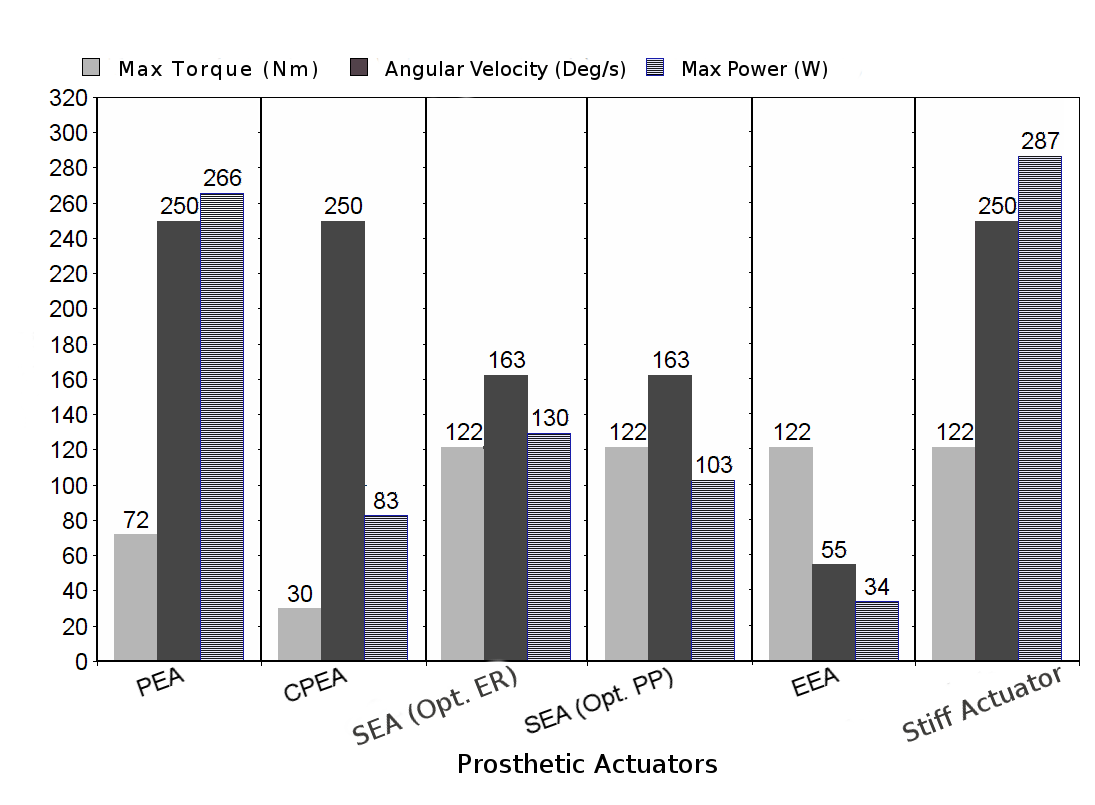
\includegraphics[scale=0.55]{20160414035751}
\par\end{centering}

\caption{\label{fig:Variables-mec=0000E1nicas-actuadores}Variables mecánicas
en actuadores protésicos para una persona de 75 kg de peso y cadencia
a 1 paso/s{\tiny{} }\cite{Cherelle2014a}. Nomenclatura: PEA: Actuador
Elástico en Paralelo, CPEA: PEA con embrague, SEA Opt RE: Actuador
Elástico en Serie optimizando el mínimo Requerimiento Energético,
SEA Opt PPi: SEA optimizando mínima Potencia Pico, EEA: Actuador Explosivo
Elástico. }
\end{figure}


Un aspecto a tener en cuenta es que la potencia energética necesaria
para realizar el empuje (\emph{push-off}) no considera las pérdidas
por la eficiencia del motor (50-60\%) y tampoco se consideran las
pérdidas energéticas por las transmisiones mecánicas de estos sistemas,
por lo que para una potencia pura de 287 W, se requieren aproximadamente
600 W reales \cite{Cherelle2014a}.

Por lo anterior, del estudio de la biomecánica de la marcha se ha
encontrado que la mayoría de la disipación de la energía ocurre cuando
el vector velocidad del COM corporal es redirigido en la transición
paso a paso. Es decir que, en cada transición el miembro posterior
en su fase de apoyo es la base para que el miembro anterior en su
fase de balanceo se comporte como un péndulo invertido, el cual transportará
el COM corporal en forma oscilante visto desde el plano sagital (Ver
Fig. \ref{fig:(A)-Representaci=0000F3n-de}A), lo anterior produce
una pérdida de energía en cada contacto inicial en la marcha en la
colisión \cite{Collins2010}. 

Por tanto, Collins y Kuo \cite{Collins2010} reciclaron esta energía
perdida a través de la compresión de un resorte metálico, para entregarla
en la fase final de apoyo (Ver Fig. \ref{fig:(A)-Representaci=0000F3n-de}C),
lo que permitió generar el trabajo positivo interno en la propulsión.
Sin embargo, no redujo la absorción al choque en ningún miembro, a
su vez el sistema no aprovechó toda la energía perdida y el empuje
fue entregado posterior a la fase terminal de apoyo.

\begin{figure}
\begin{centering}
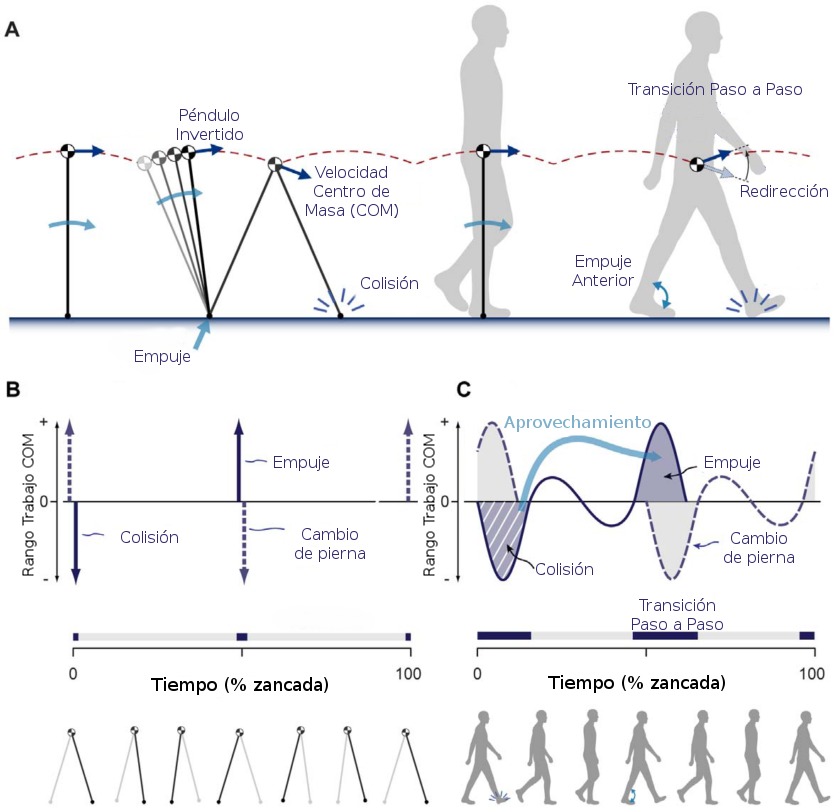
\includegraphics[scale=0.57]{Recycled}
\par\end{centering}

\caption{\label{fig:(A)-Representaci=0000F3n-de}(A) Representación de la fase
de apoyo en la marcha comportándose como un péndulo invertido, se
aprecia el re-direccionamiento del vector velocidad del COM. (B) Tasa
de trabajo de cada pierna durante la longitud de la zancada generada
por el COM, la diferencia de distancia entre vectores indica la transición
del trabajo en cada paso. (C) Representación teórica de la tasa de
trabajo de cada miembro vs. la longitud de la zancada, el propósito
es aprovechar el trabajo negativo perdido en el impacto de talón y
retornarlo en la fase de propulsión \cite{Collins2010}.}


\end{figure}


A grandes rasgos las prótesis activas siguen un mismo procedimiento
de diseño: utilizan un pie pasivo, implementan un actuador para la
propulsión en la dorsiflexión máxima del pie, aplican una estrategia
de control para la marcha y una fuente de energía abastecerá su funcionamiento.
Por lo que surge la incógnita de incursionar en otras estrategias
que puedan suplir la necesidad de los amputados de una manera más
eficiente.

Si bien en el campo de la protésica y de la ingeniería se están realizando
aproximaciones para mimetizar las funciones del triceps surae, algunas
otras como la de \cite{Takahashi2013} se enfocan en las contribuciones
de la parte distal del pie, las cuales no se han replicado a la fecha
a causa de su aporte en trabajo negativo.

En síntesis, las patologías presentadas en amputaciones de miembros
inferiores se traducen en afectaciones energéticas al usuario (costo
metabólico), dada la ausencia del 80\% del trabajo neto generado por
el triceps surae, y del porcentaje restante del trabajo generado por
los músculos intrínsecos y tejidos del pie.

En consecuencia de lo anterior, se presentan alteraciones en los patrones
de marcha a falta de trabajo positivo en la dorsiflexión y baja absorción
al choque en prótesis pasivas. Por ende, las investigaciones en protésica
se han enfocado al desarrollo de actuadores protésicos para poder
subsanar las patologías presentes aún en prótesis ESR. Para una mejor
ilustración de la problemática se presenta el \nameref{sec:Ap=0000E9ndice-C}.

Sin embargo, la baja eficiencia de los actuadores implementados a
la fecha afectan la autonomía de las prótesis activas, sin descartar
los demás inconvenientes mencionados anteriormente en esta clase de
prótesis. Por tanto surge la necesidad de incursionar en el diseño
de sistemas \emph{dinámicos pasivos} \cite{mcgeer1990passive} para
la protésica de miembros inferiores que aprovechen la energía mecánica
a disipar en la colisión del contacto inicial y devolverla en la dorsiflexión
máxima (Ver Fig. \ref{fig:Gr=0000E1fica-de-torque}), sin
afectar el espacio antropométrico del miembro ausente. Lo anterior
permitirá subsanar las alteraciones presentes con prótesis pasivas
y brindará un trabajo positivo interno mayor al que generan éstas.


\subsection*{Manufactura aditiva en prótesis:}

El desarrollo tecnológico en manufactura ha sido aprovechado en el
campo de la medicina, desde la fabricación de dispositivos con fines
de enseñanza hasta la reproducción de una célula, un tejido, un órgano
y/o un implante \cite{Michalski2014}. Todo se debe a la revolución
industrial del 3D printing o manufactura aditiva, la cual forma la
pieza o conjunto capa por capa sin necesidad de remover material a
partir de un modelo CAD\nomenclature{CAD}{Diseño Asistido por Computador}.

La tecnología en \emph{Manufactura Aditiva} (\nomenclature{MA}{Manufactura Aditiva}MA)
o impresión 3D (3D printing) brinda muchas ventajas en comparación
a los métodos de fabricación convencionales, las cuales se detallan
en los estudios de Weller \emph{et al.} \cite{Weller2015} y Diegel
\emph{et al.} \cite{Diegel2014}. Estas bondades han sido aprovechadas
por diversos investigadores en prótesis para fabricar sus modelos
experimentales, tal es el caso de South \emph{et al.}\cite{South2010}
que determinó el efecto de la rigidez de la prótesis de pie pasiva
en los parámetros biomecánicos del usuario, usando el método de sinterizado
por láser para la fabricación. Otro caso más reciente es el de Yap
\emph{et al.} \cite{Yap2015}, cuyo propósito era fabricar una prótesis
con diferentes antropometrías para que los pacientes pediátricos se
adapten a este dispositivo a medida que vayan creciendo. En miembros
superiores el prototipo biomimético más destacado es el de Xu y Todorov
\cite{Xu2016}, cuya geometría del modelo fue tomada de una mano esquelética
real.

Ahora bien, la tecnología en MA y el concepto de auto-ensamblaje lograron
fabricar dispositivos que cambian de forma con el tiempo, a esto se
le conoce como impresión 4D. Estos modelos cambian de forma una vez
se les somete a un cambio de ambiente pasivo (e.g., inmersión en agua
\cite{Tibbits2014,Raviv2014}, cambios de temperatura \cite{Yu2015}),
a su vez se puede manipular la elasticidad del modelo gracias a la
capacidad de imprimir en diferentes materiales las secciones deseadas.

Lo anterior es muestra de que los materiales para impresión 3D cuentan
con la suficiente capacidad mecánica estructural para fabricar modelos
de este tipo, a su vez esta tecnología brinda una mayor libertad en
cuanto a la geometría de las piezas se refiere.

Si bien se han realizado dispositivos protésicos en impresión 3D para
miembros inferiores, estos modelos manejan propiedades mecánicas del
material uniformes, sabiendo que para obtener una aproximación real
del tobillo se deben poder controlar las propiedades visco-elásticas
(aunque en ciertas instancias la contribución viscosa en la marcha
normal es nula \cite{Hansen2004}) y elásticas de las distintas zonas
que conforman el mismo para obtener la \emph{cuasi-rigidez} del sistema. 

Dada la habilidad de la impresión 3D para adicionar material libremente,
ésta puede tener gran impacto en cómo puede ser diseñado un objeto
o conjunto dependiendo de las propiedades mecánicas deseadas. A su
vez, teniendo en cuenta que la estrategia del diseño del prototipo
de prótesis es proveer diferentes configuraciones elásticas en el
modelo para almacenar la mayor cantidad de energía posible y posteriormente
proveerla en un instante específico, surge la posibilidad de implementar
materiales celulares en la configuración deseada.

Los materiales celulares pueden alcanzar alta rigidez y resistencia
por unidad de masa, a su vez, pueden proveer buenas características
de absorción de energía \cite{Gibson1997}. Los materiales celulares
incluyen varias geometrías, tales como: espumas, panal de abejas y
configuraciones enrejadas (\emph{lattice}).

Su implementación con MA ha mostrado buenos resultados en cuanto a
la fabricación de distintos tipos de sólido celular, bien sea en la
obtención de un meta-material para el control de la rigidez a medida
que el material se somete a una tensión \cite{Wang2016}, o para la
obtención de la rigidez deseada en diferentes secciones a través de
la implementación de algoritmos de optimización \cite{Chu2010}.

Sin embargo, predecir el comportamiento de estos materiales desde la experimentación conlleva una alta relación costo-beneficio, a su vez ciertas variables (i.e. plasticidad cristalina, mecánica macro-molecular, distorsión de las células, entre otros.) no son fácilmente observables mediante la experimentación \cite{Okereke2014}.

Para ello, distintas pruebas virtuales se han llevado a cabo con este tipo de materiales mediante la técnica FEM, las cuales han sido validadas mediante la experimentación. Tal es el caso de Heimbs \cite{Heimbs2009}, el cual determinó el comportamiento dinámico \emph{In silico} de cuatro diferentes configuraciones de estructuras \emph{honeycomb} a diferentes tipos de carga compresiva (i.e. \emph{In-plane} y \emph{Out-of-plane}). El estudio determinó cuáles son las principales variables influyentes para una buena correlación con los resultados experimentales (Ver Fig. \ref{fig:CellularFEM}A).

\begin{figure}
\begin{centering}

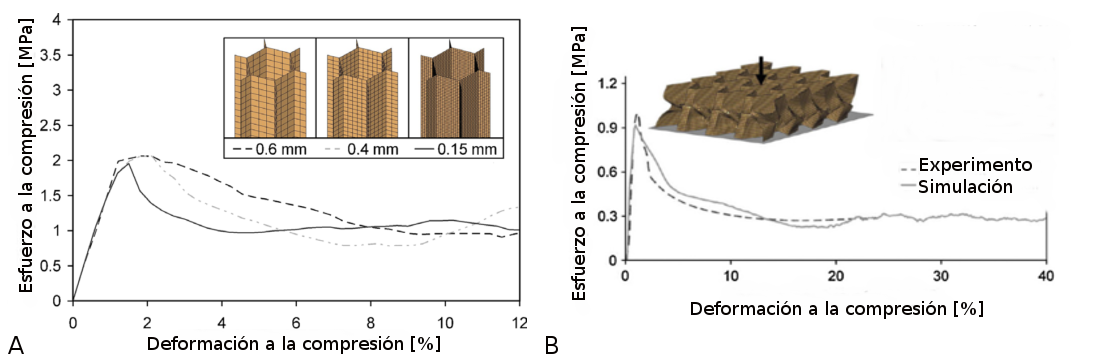
\includegraphics[scale=0.45]{stress-strainFEM2}
\par\end{centering}

\caption{\label{fig:CellularFEM} A) Resultados del esfuerzo a la compresión de una configuración estructural tipo \emph{honeycomb} mediante una carga \emph{Out-of-plane} con diferentes refinamientos en el mallado. B) Curva esfuerzo-deformación a la compresión de una estructura \emph{Honeycomb} obtenida \emph{In-silico}, comparada con los resultados experimentales. Editado de Heimbs \cite{Heimbs2009}}
\end{figure}

Otras técnicas similares que no se consideran sólidos celulares pero si conservan el mismo propósito son las micro-estructuras a pequeña escala, cuya obtención de las propiedades mecánicas, dependerán de
su geometría y respectivas configuraciones internas, más no de las
propiedades del material \cite{Schumacher2015}.


\subsection*{Modelos computacionales músculo-esqueléticos:}

Algunos parámetros biomecánicos previamente mencionados no son fáciles
de medir o estimar a simple vista, del mismo modo, algunos prototipos
de prótesis (e.g., \cite{Lapre2014}) no fueron validados en paciente
sin pasar por una verificación computacional que asegure el cumplimiento
de los requerimientos de diseño. 

Por tanto, una buena estrategia para dilucidar la relación entre la
estructura fisiológica y el comportamiento biomecánico a estudiar
es el método del modelado computacional. Aunque las simplificaciones
biológicas, físicas y de ingeniería no aseguran un comportamiento
completamente certero, estas brindan ciertas ventajas al momento de
realizar experimentaciones en el modelo, como son: i) La habilidad
para predecir un efecto o respuesta; ii) Habilidad para estimar parámetros
que son imposibles o difíciles de medir a simple vista; iii) Libertad
desde el punto de vista de las restricciones éticas en experimentaciones
con seres vivos, entre otros \cite{Talaty2014}.

La evolución de los modelos de marcha bípeda los describe Cifuentes
\emph{et al.} \cite{Cifuentes2010}, donde se encontró que el modelo
de marcha humana más aproximado a los requerimientos del presente
trabajo es Opensim$\circledR$\cite{Delp2007,Reinbolt2011,Seth2011}.
Este software permite realizar simulaciones dinámicas del movimiento
corporal a través de la integración de los siguientes desarrollos
previos: 
\begin{itemize}
\item SIMM: \emph{(Software for Interactive Musculoskeletal Modeling}) Ésta
herramienta facilita el modelado, la visualización y el análisis
del sistema músculo-esquelético visto en 3D. Algunos modelos (e.g.,\cite{Arnold2010})
cuentan con una caracterización antropomórfica robusta del sistema
músculo-tendinoso y esquelético para poder ser usados en casos específicos
una vez realizada la escalización de cada uno.
\item Simbody \cite{Sherman2011}: API \emph{(Application Programming Interface)}
para realizar simulaciones de modelos coordenados de sistemas multicuerpo.
La librería de programación le permite realizar análisis dinámicos
para aplicaciones biomédicas a diferentes escalas.
\end{itemize}
Al desear subsanar las alteraciones biomecánicas presentes en un usuario
de prótesis pasiva en la marcha humana es necesario cuantificar los
parámetros cinemáticos y cinéticos del estudio de caso, para poder
calcular posteriormente el ciclo de trabajo tanto interno (a través
de la cinemática inversa) como externo (a través de la plataforma
de fuerzas) de la prótesis de referencia, como del nuevo concepto
a plasmar. La viabilidad para su realización es alta debido a la experiencia del candidato y del grupo de investigación GIBM-UNCB en la temática, éste bagaje puede apreciarse en el \nameref{sec:Ap=0000E9ndice-A}.




\section*{IDENTIFICACIÓN DEL PROBLEMA}
\begin{itemize}
\item Las prótesis pasivas actuales utilizadas en pacientes con amputación transtibial, provocan alteraciones en los parámetros dinámicos de la marcha, debido a la ausencia de trabajo positivo del miembro faltante.
\end{itemize}

\subsection*{Pregunta de investigación: }

¿Qué configuración de prótesis transtibial pasiva, generará el trabajo
positivo necesario en la fase de apoyo final, a través del aprovechamiento
de la energía perdida del Contacto Inicial de la marcha?


\subsection*{Hipótesis:}

Una prótesis transtibial, configurada para aprovechar la energía perdida
del Contacto Inicial, permitirá generar el trabajo positivo necesario
en la fase de apoyo final a través de un sistema dinámico pasivo.



\section*{OBJETIVO GENERAL Y ESPECÍFICOS}
\begin{description}
\item [{Objetivo}] \textbf{General:} Proponer una configuración de prótesis
transtibial, que genere a través de un sistema dinámico pasivo, el
trabajo positivo necesario en la dorsiflexión máxima, aprovechando
la energía perdida en el contacto inicial de la marcha.
\item [{Objetivos}] \textbf{Específicos:}\end{description}
\begin{enumerate}
\item Identificar los parámetros biomecánicos y el diagrama del ciclo de
trabajo a usuarios de prótesis pasivas con amputación unilateral
transtibial para determinar sus requerimientos energéticos.
\item Obtener el modelo preliminar de la prótesis transtibial que
aproveche la energía, durante el contacto inicial y el apoyo medio,
para entregarla en la fase de apoyo final de la marcha mediante un
sistema dinámico pasivo.
\item Determinar la configuración detallada del modelo preliminar de prótesis transtibial mediante la aplicación de sólidos celulares.
\item Validar el modelo dinámico de la prótesis transtibial configurada,
en comparación a un modelo protésico pasivo.\end{enumerate}
\begin{description}
\item [{METODOLOGÍA Y ACTIVIDADES:}]
\end{description}
El procedimiento metodológico general se llevará a cabo mediante una parte experimental (adquisición de datos dinámicos en la marcha y validación del modelo) y otra parte \emph{In-Silico}, donde se llevará el proceso de diseño y verificación del funcionamiento de la prótesis. La metodología computacional se concentrará en un marco construido en lenguaje Python, tal como lo muestra la Fig. \ref{Marco-computacional}. A su vez, todo el proceso computacional pasará por el proceso de validación propuesto por Hicks \emph{et al.} \cite{Hicks2014}, el cual se muestra en la Fig. \ref{fig:Proceso-validaci=0000F3n-y}.

Ahora, para cada objetivo se presenta una metodología particular, sin obviar la organización anteriormente mencionada, por tanto se presenta la siguiente metodología y actividades particulares, así:
\begin{figure}[ht]
\begin{centering}
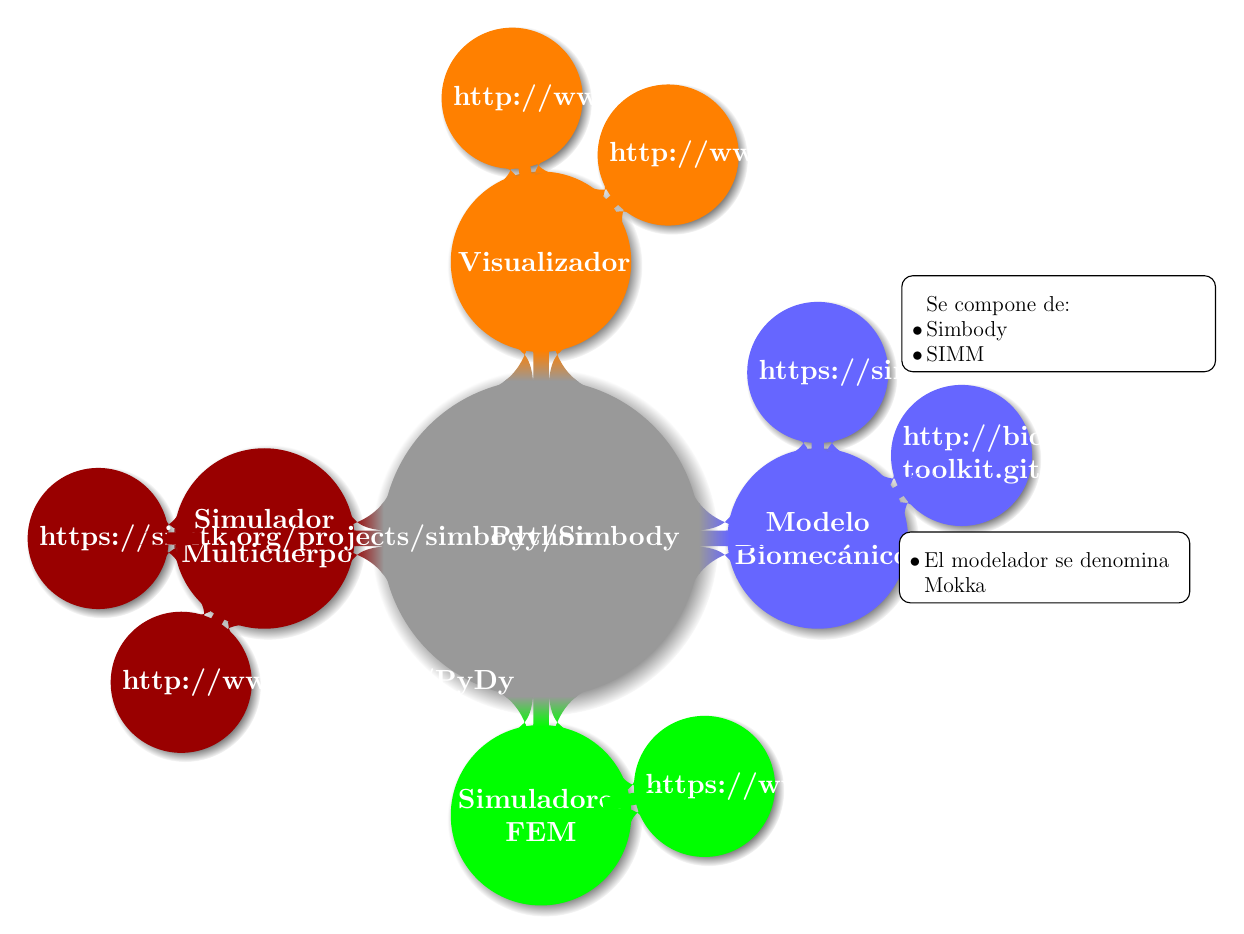
\begin{tikzpicture}[ every annotation/.style = {draw,
                     fill = white, font = \large,text width=4em}]
  \path[mindmap,concept color=black!40,text=white,
    every node/.style={concept,circular drop shadow},
    root/.style    = {concept color=black!40,
      font=\normalsize\bfseries,text width=6em},
    level 1 concept/.append style={font=\normalsize\bfseries,
      sibling angle=90,text width=6em,
    level distance=10em,inner sep=0pt},
    level 2 concept/.append style={font=\bfseries,level distance=6em},
  ]
  node[root] {Python} [clockwise from=0]
    child[concept color=blue!60] {
      node {{Modelo Biomecánico}} [clockwise from=90]
        child { node (goForum) {\href{https://simtk.org/projects/opensim}{Opensim}} }
        child { node (goWiki) {\href{http://biomechanical-toolkit.github.io/}{BTK}} }
    }
    child[concept color=green!120] {
      node[concept] {{Simuladores FEM}}
        [clockwise from=10]
      child { node[concept] {\href{https://www.csc.fi/web/elmer}{ELMER}} }
    }
    child[concept color=red!60!black] {
      node[concept] {{Simulador Multicuerpo}}
        [counterclockwise from=180]
      child { node[concept] {\href{https://simtk.org/projects/simbody/}{Simbody}}}
      child { node[concept] {\href{http://www.pydy.org/}{PyDy}} }
      }
    child[concept color=orange] {
      node[concept] {{Visualizador}}
        [clockwise from=100]
        child { node[concept] {\href{http://www.vtk.org/documentation/}{VTK}}
        }
        child { node[concept] {\href{http://www.paraview.org/overview/}{Paraview}}
        }};
    \info{goForum.north east}{above,anchor=west,xshift=1em}{%
      \item[] Se compone de:
      \item Simbody
      \item SIMM
    }
    \info[15]{goWiki.south}{below,anchor=north,xshift=3em}{%
      \item El modelador se denomina Mokka
    }

\end{tikzpicture}
\caption{\label{Marco-computacional} Marco computacional de la metodología. Los hiper-vínculos direccionan a la página principal de cada programa tentativo \emph{Open-source} a implementar en el proyecto. }
\end{centering}
\end{figure}
\begin{figure}[ht]
\begin{centering}
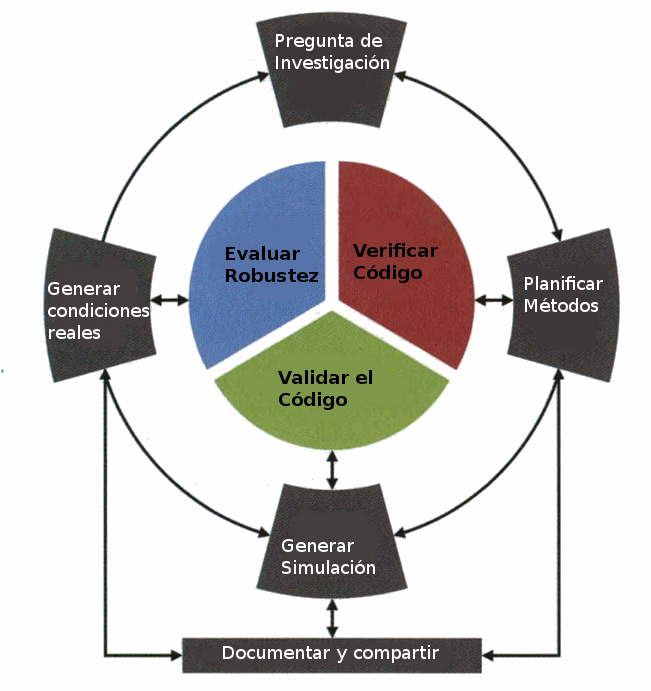
\includegraphics[scale=0.5]{verificationprocess}
\par\end{centering}

\caption{\label{fig:Proceso-validaci=0000F3n-y}Proceso validación y verificación
modelos biomecánicos de Hicks \emph{et al.} \cite{Hicks2014}}
\end{figure}
\begin{description}
\item [{Objetivo}]  \textbf{1:} Identificar los parámetros biomecánicos
y el diagrama del ciclo de trabajo a usuarios de prótesis pasivas
con amputación unilateral transtibial para determinar sus requerimientos
energéticos.
\item [{Metodología:}] Adquirir los principales parámetros biomecánicos
(Ver Tabla. \ref{tab:Principales-par=0000E1metros-usados}) de la marcha
normal para obtener el modelo biomecánico de un usuario de prótesis
ESR con amputación transtibial unilateral y otro sujeto sin patologías
(de antropometría similar) como referencia.
\end{description}
\begin{table}[H]
\caption{\label{tab:Principales-par=0000E1metros-usados}Principales parámetros
según Sagawa \emph{et al.} \cite{Sagawa2011}, utilizados para el
análisis de la marcha en amputados de miembro inferior.}


\noindent \centering{}%
\begin{tabular}{|>{\raggedright}m{5cm}|>{\centering}p{9cm}|}
\hline 
\multirow{9}{5cm}{ \textbf{Parámetros Espacio-temporales}} & Velocidad (m/s)\tabularnewline
\cline{2-2} 
 & Cadencia (pasos/min)\tabularnewline
\cline{2-2} 
 & Tiempo del ciclo completo (s)\tabularnewline
\cline{2-2} 
 & Tiempo fase de apoyo (s)\tabularnewline
\cline{2-2} 
 & Tiempo fase de balanceo (s)\tabularnewline
\cline{2-2} 
 & Tiempo en el apoyo simple (s)\tabularnewline
\cline{2-2} 
 & Tiempo en el apoyo doble (s)\tabularnewline
\cline{2-2} 
 & Longitud del paso (m)\tabularnewline
\cline{2-2} 
 & Localización del COM respecto al piso\tabularnewline
\hline 
\multirow{3}{5cm}{ \textbf{Ángulos articulares}} & Ángulos de cadera (rad)\tabularnewline
\cline{2-2} 
 & Ángulos de rodilla (rad)\tabularnewline
\cline{2-2} 
 & Ángulos de tobillo (rad)\tabularnewline
\hline 
\multirow{3}{5cm}{\textbf{Momentos articulares}} & Cadera (Nm/kg)\tabularnewline
\cline{2-2} 
 & Rodilla (Nm/kg)\tabularnewline
\cline{2-2} 
 & Tobillo (Nm/kg)\tabularnewline
\hline 
\multirow{3}{5cm}{ \textbf{Potencia Articular}} & Cadera (W/kg)\tabularnewline
\cline{2-2} 
 & Rodilla (W/kg)\tabularnewline
\cline{2-2} 
 & Tobillo (W/kg)\tabularnewline
\hline 
\multirow{4}{5cm}{\textbf{Plataforma}} & Fuerza de Reacción anteroposterior\tabularnewline
\cline{2-2} 
 & Fuerza de reacción vertical\tabularnewline
\cline{2-2} 
 & Impulso de reacción anteroposterior\tabularnewline
\cline{2-2} 
 & Centro de Presiones (COP)\tabularnewline
\hline 
\end{tabular}
\end{table}

\begin{description}
%\vspace{10 mm}
\item [{Actividades:}]~\end{description}
\begin{enumerate}
\item Solicitar la respectiva autorización al comité de ética para dar aval
al estudio en laboratorio de marcha a los sujetos con y sin alteraciones dinámicas.
\item Realizar el procedimiento para adquirir los parámetros biomecánicos
(Ver Tabla. \ref{tab:Principales-par=0000E1metros-usados}) en laboratorio
de marcha a un usuario con prótesis
ESR amputado unilateral y a un usuario sin patologías a marcha
normal para tomarlo como referencia.
\item Obtener el modelo biomecánico computacional de los sujetos objeto
del estudio, con el propósito de adquirir los parámetros no cuantificables
directamente en laboratorio a través de la dinámica inversa y posteriormente
la dinámica directa, mediante una herramienta \emph{Open-source } biomecánica (e.g.
Opensim$\circledR$).
\item Obtener la magnitud de energía perdida en la colisión y la cuasi-rigidez
de la articulación de tobillo en los casos de estudio a través de
los datos obtenidos en la plataforma de fuerzas y dinámica inversa
respectivamente.
\item Realizar el proceso de verificación de la dinámica del modelo biomecánico computacional mediante la comparación de estudios similares publicados en la literatura.\end{enumerate}
\begin{description}
\item [{Objetivo}]  \textbf{ 2: }Obtener el modelo preliminar de la configuración
de prótesis transtibial que aproveche la energía, durante el contacto
inicial y el apoyo medio, para entregarla en la fase de apoyo final
de la marcha mediante un sistema dinámico pasivo.
\item [{Metodología:}] A través de herramientas para simulación dinámica
multi-cuerpo deformable combinada con FEM, proponer la configuración del sistema global de la prótesis mediante el fraccionamiento del espacio antropométrico, con el fin de acumular la energía mediante deformación elástica en determinados sub-dominios y a su vez brindar estabilidad estructural al sistema.
\end{description}

\begin{description}
\item [{Actividades:}]~\end{description}
\begin{enumerate}
\item Separar el modelo dinámico de cuerpos rígidos (obtenido del Objetivo 1), de acuerdo a las sub-fases mostradas en la cuasi-rigidez (Ver Fig. \ref{fig:Cuasi-rigidez-de-la}) para cada estudio de caso (Opensim$\circledR$).
\item Definir la geometría o dominio global de acuerdo a una aproximación
antropomórfica de la zona transtibial del modelo amputado (Inventor$\circledR$).
\item Definir la configuración elástica necesaria para el almacenamiento energético en las sub-fases de Contacto Inicial y Dorsiflexión máxima (Simbody$\circledR$).
\item Definir la configuración de los sub-dominios rígidos para dar estabilidad estructural en el CI y despegue de pie (Simbody$\circledR$).
\item Fraccionar el dominio total y proponer la ecuación constitutiva para cada sub-dominio de acuerdo a los requerimientos elásticos obtenidos en el anterior modelo. (PyDy$\circledR$/Simbody$\circledR$ y ELMER$\circledR$).
\item Diseñar el sistema que encapsule la energía del Contacto
Inicial y la entregue en la fase de apoyo terminal. (Simbody$\circledR$).
\item Realizar la simulación dinámica multicuerpo deformable combinada con FEM del modelo. (ELMER$\circledR$).
\item Verificar que el modelo almacene la energía durante la fase de apoyo
y el sistema dinámico la libere (Opensim$\circledR$ y ELMER$\circledR$).\end{enumerate}
\begin{description}
\item [{Objetivo}]  \textbf{ 3: }Determinar la configuración detallada del modelo preliminar de prótesis transtibial mediante la aplicación de sólidos celulares.
\item [{Metodología:}] De la configuración obtenida del modelo multi-cuerpo para cada subdominio, se debe implementar un material equivalente tal
que cumpla con las propiedades elásticas del modelo anterior, para
ello la propuesta es implementar sólidos celulares y la forma de verificar
su comportamiento se realizará a través de simulaciones FEM y/o DES.
\item [{Actividades:}]~\end{description}
\begin{enumerate}
\item Configurar el sólido celular de acuerdo a las propiedades
elásticas específicas de cada subdominio obtenido en el modelo obtenido en el objetivo 2.
\item Verificar el comportamiento del sólido celular en cada sub-dominio, de acuerdo a su respuesta constitutiva (e.g curva esfuerzo-deformación) mediante cargas cuasi-estáticas ó dinámicas, determinadas en las condiciones de frontera. (ELMER$\circledR$).
\item Verificar la resistencia estructural estática del modelo entero, de acuerdo
a las sub-fases de mayor carga, estas son Contacto Inicial y Dorsiflexión
máxima mediante técnicas de simulación \nomenclature{FEM}{\emph{Finite Element Method} / Método por Elementos Finitos}FEM
o FEM/DES\nomenclature{DES}{\emph{Discrete Element Method} / Método por Elementos Discretos}. (ELMER$\circledR$).
\item Obtener el ciclo de trabajo de la nueva configuración mediante la
dinámica directa del modelo biomecánico anterior. (Opensim$\circledR$ y ELMER$\circledR$)
\end{enumerate}
\begin{description}
\item [{Objetivo}]  \textbf{ 4:}Validar el modelo dinámico de la prótesis
transtibial configurada, en comparación a un modelo protésico pasivo.
\item [{Metodología:}] Realizar la impresión 3D del modelo obtenido y validar el trabajo positivo generado del nuevo concepto mediante pruebas de marcha,
comparándolos a su vez con un usuario sin patologías.
\item [{Actividades:}]~\end{description}
\begin{enumerate}
\item Adaptar al usuario objeto del estudio, al manejo y utilización de
la prótesis una vez su adaptación se haya completado.
\item Adquirir los parámetros biomecánicos del usuario con el nuevo prototipo
y con su prótesis cotidiana pasiva.
\item Realizar la comparación del trabajo positivo generado durante la transición paso a paso de los tres casos de referencia (patológico con ESR, patológico con el nuevo concepto y no patológico)
\item Determinar la energía almacenada por el prototipo de acuerdo a la deformación del modelo, mediante un sistema de medición óptico (e.g. \href{http://www.gom.com/industries/medical-technology/biomechanics.html}{GOM}).
\item Evaluar las diferencias significativas en cada instancia de la fase
de apoyo en la marcha y emitir conclusiones.
\end{enumerate}

\section*{IMPLICACIONES Y RESULTADOS ESPERADOS:}

\subsection*{Implicaciones e impacto en la investigación:}

El impacto en la investigación radica en el planteamiento de un nuevo
concepto de prótesis transtibial capaz de almacenar la energía en
la colisión y en la dorsiflexión para retornarla de una manera controlada en la fase terminal de apoyo, aumentando la contribución energética en comparación a las prótesis pasivas ya existentes.

Por otro lado, la cuasi-rigidez de la articulación de tobillo depende directamente
del peso y de la longitud del paso, lo cual genera una necesidad de
personalización en una prótesis transtibial, a su vez las propiedades
mecánicas uniformes de las prótesis pasivas actualmente existentes
no permiten una mimetización detallada de la articulación, lo cual
genera demanda metabólica mucho mayor a la de una persona sin ésta
patología. Por otro lado, las prótesis activas generan el trabajo
positivo requerido pero con una ineficiencia alta, lo cual genera
problemas de autonomía con la prótesis, a su vez su arquitectura electrónica
hace de estos dispositivos prácticamente inalcanzables a los usuarios
de países del tercer mundo por su alto costo.

A su vez, con los métodos de fabricación planteados, se puede generar una metodología para personalizar la configuración protésica de acuerdo a los parámetros biomecánicos de la persona, la cual tendrá una configuración interna mediante sólidos celulares o micro-estructuras
para alcanzar propiedades específicas de elasticidad en su prótesis.

\subsection*{Resultados esperados: }
\begin{table}[H]
\begin{centering}
\caption{Resultados esperados de la investigación}
\begin{tabular}{|>{\centering}m{5cm}|>{\centering}p{7cm}|>{\centering}p{3cm}|}
\hline 
Entregable & Resultado esperado & Probabilidad \tabularnewline
\hline 
\hline 
Artículo publicable en revista indexada: \emph{Computers in Biology
and Medicine, Journal of biomechanical engineering o SAGE.} & Un modelo dinámico multi-cuerpo que emule y verifique la generación del trabajo positivo necesario para un amputado unilateral
transtibial con el sistema protésico transtibial planteado. & Alta\tabularnewline
\hline 
\multirow{2}{5cm}{Artículo publicable en revista indexada: \emph{Rapid Prototyping Journal,
Journal of Mechanical Design o Journal of the mechanical behaviour
of biomedical materials.}} & Resultado experimental de la comparación de los parámetros dinámicos en la marcha con el prototipo de prótesis transtibial personalizada vs. prótesis ESR vs. usuario sin patologías.
aditiva. & Alta\tabularnewline
\cline{2-3} 
 & Metodología de personalización para amputados de miembro inferior. & Media\tabularnewline
\hline 
Solicitud de patente o modelo de utilidad ante la SIC. & Que sea fabricable mediante técnicas de manufactura aditiva para habilitar
la posibilidad de escalar el sistema para varias antropometrías con
mayor facilidad. & Media\tabularnewline
\hline 
Prototipo de prótesis transtibial personalizada. & Un modelo basado en estructuras celulares ayudará a subsanar las anormalidades
en los parámetros biomecánicos del usuario objeto del estudio. & Alta\tabularnewline
\hline 
\end{tabular}
\end{centering}
\end{table}
\vspace{2cm}
\begin{sidewaysfigure}
\begin{centering}
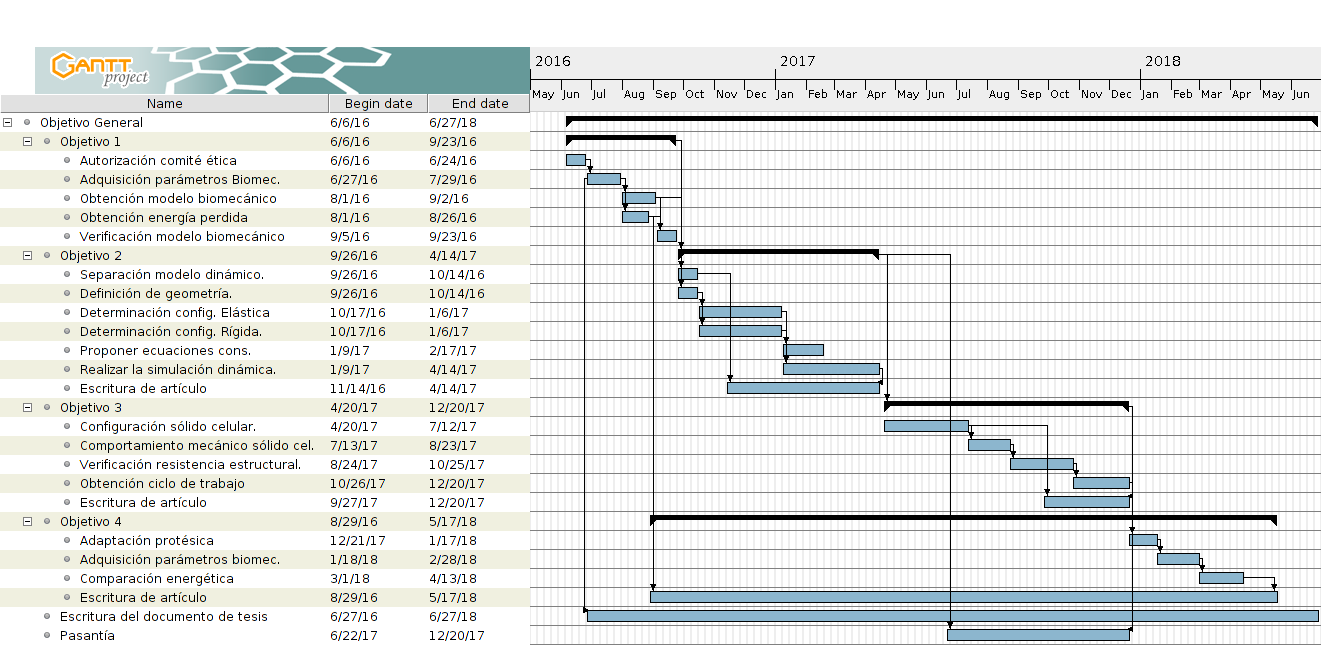
\includegraphics[scale=0.52]{Cronograma}
\par\end{centering}

\caption{Cronograma de actividades}


\end{sidewaysfigure}


\renewcommand\refname{BIBLIOGRAPHY}
%\begin{verse}
\bibliographystyle{ieeetr}
\bibliography{Proposal,patents}
%\end{verse}
\begin{description}
\item [{RECURSOS}]  \textbf{FÍSICOS:}(Especificar la disponibilidad y
adjuntar carta de compromiso de la dependencia o empresa cuando sea
necesario).
\item [{COSTOS}]  \textbf{DEL TRABAJO Y FUENTES DE FINANCIACIÓN:}
\end{description}
\begin{table}[H]
\caption{Presupuesto global de la propuesta de investigación. }
\noindent \begin{centering}
\begin{tabular}{|>{\centering}p{40mm}|>{\centering}p{30mm}|>{\centering}p{35mm}|>{\centering}p{30mm}|}
\hline 
\multirow{2}{40mm}{\textbf{Rubro}} & \multicolumn{2}{c|}{\textbf{Fuente}} & \multirow{2}{30mm}{\textbf{Subtotal}}\tabularnewline
\cline{2-3} 
 & \textbf{Interna} & \textbf{Externa} & \tabularnewline
\hline 
\hline 
\textbf{Personal} & \$26.319.000.00{*} & \$144.000.000.00\lyxarrow{} & \$170.319.000.00\tabularnewline
\hline 
\textbf{Equipo} & \$ 9.500.000.00{*} &  & \$ 9.500.000.00\tabularnewline
\hline 
\textbf{Materiales} &  & \$10.000.000.00{*}{*} & \$10.000.000.00\tabularnewline
\hline 
\textbf{Salidas de campo} &  & \$ 5.000.000.00{*}{*} & \$ 5.000.000.00\tabularnewline
\hline 
\textbf{Capacitación} &  & \$ 41.600.000.00\lyxarrow{} & \$ 41.600.000.00\tabularnewline
\hline 
\textbf{Publicaciones y patentes} &  & \$5.000.000.00{*}{*} & \$5.000.000.00\tabularnewline
\hline 
\textbf{Servicios Técnicos} &  & \$10.000.000.00{*}{*} & \$ 10.000.000.00\tabularnewline
\hline 
\textbf{Viajes} &  & \$4.000.000.00\lyxarrow{} & \$4.000.000.00\tabularnewline
\hline 
\textbf{Total} & \$ 35.819.000.00 & \$ 219.600.000.00 & \$ 255.419.000.00\tabularnewline
\hline 
\end{tabular}
\par\end{centering}


\begin{lyxlist}{00.00.0000}
\item [{Nota:}] Los rubros marcados con ({*}) se determinaron de acuerdo
al cálculo del sistema Hermes y estarían cubiertos como contrapartida
interna en especie. Los rubros marcados con ({*}{*}) son presupuestos no aprobados
por el momento, los cuales se solicitarán a través de un proyecto
COLCIENCIAS, convocatoria interna y/o convocatorias Banco de la República. Los presupuestos marcados con (\lyxarrow{}) están cubiertos por la convocatoria para conformar bancos de elegibles para formación de alto nivel para la ciencia, la tecnología y la innovación de COLCIENCIAS.\end{lyxlist}
\end{table}


\begin{table}[H]
\caption{Descripción de gastos de personal}
\noindent \begin{centering}
{\small{}}%
\begin{tabular}{|>{\raggedright}m{5cm}|>{\raggedright}m{22mm}|>{\raggedright}m{10mm}|>{\raggedright}m{14mm}|>{\centering}p{27mm}|>{\centering}p{27mm}|}
\hline 
\multirow{2}{5cm}{{\footnotesize{} \textbf{Nombre del Investigador}\vspace{30 mm}}} & \multirow{2}{22mm}{{\footnotesize{} \textbf{Vinculación con la UNAL}}} & \multirow{2}{10mm}{{\footnotesize{} \textbf{No. meses}}} & \multirow{2}{14mm}{{\footnotesize{} \textbf{Horas / Semana}}} & \multicolumn{2}{c|}{{\footnotesize{} \textbf{Recursos}}}\tabularnewline
\cline{5-6} 
 &  &  &  & {\footnotesize{} \textbf{Internos}} & {\footnotesize{} \textbf{Externos}}\tabularnewline
\hline 
{\small{}Dr. Ing. Carlos Julio Cortés R.} & {\small{}Tiempo Completo} & {\small{}48} & {\small{}3} & {\small{}\$ 14.661.000.00} & \tabularnewline
\hline 
{\small{}Ing. Edwin Nikolay Prieto P. } & {\small{}Becario COLCIENCIAS} & {\small{}48} & {\small{}48} &  & {\small{}\$144.000.000.00}\tabularnewline
\hline 
{\small{}MD. Octavio Silva Caicedo} & Tiempo Completo & {\small{}36} & {\small{}1} & \$11.658.000.00 & \tabularnewline
\hline 
{\small{} \textbf{Subtotal}} &  &  &  & {\small{}\$ 26.319.000.00} & {\small{}\$144.000.000.00}\tabularnewline
\hline 
\end{tabular}
\par\end{centering}{\small \par}


\end{table}


\begin{table}[H]
\caption{Descripción de los equipos estimados a adquirir.}
\noindent \begin{centering}
\begin{tabular}{|>{\raggedright}p{3cm}|>{\raggedright}p{4cm}|>{\centering}p{3cm}|>{\centering}p{3cm}|}
\hline 
\multirow{2}{3cm}{\textbf{Equipo}} & \multirow{2}{4cm}{\textbf{Justificación}} & \multicolumn{2}{>{\centering}p{4cm}|}{\textbf{Recursos}}\tabularnewline
\cline{3-4} 
 &  & Interno & Externo\tabularnewline
\hline 
Computador de Escritorio & Elemento necesario para realizar el modelado y análisis computacional. & \$ 7.000.000.00 & \tabularnewline
\hline 
Computador portátil & Necesario para procesamiento de datos e informes. & \$ 2.500.000.00 & \tabularnewline
\hline 
{\small{} \textbf{Subtotal}} &  & \$ 9.500.000.00 & \tabularnewline
\hline 
\end{tabular}
\par\end{centering}

\end{table}


\begin{table}[H]
\caption{Descripción de materiales estimados a adquirir.}
\begin{centering}
\begin{tabular}{|>{\raggedright}p{3cm}|>{\raggedright}p{4cm}|>{\raggedright}p{2cm}|>{\centering}p{3cm}|>{\centering}p{3cm}|}
\hline 
\multirow{2}{3cm}{\textbf{Material}} & \multirow{2}{4cm}{\textbf{Justificación}} & \multirow{2}{2cm}{\textbf{Cantidad}} & \multicolumn{2}{c|}{\textbf{Recursos}}\tabularnewline
\cline{4-5} 
 &  &  & Interno & Externo\tabularnewline
\hline 
Material para Manufactura Aditiva & Para realizar modelos a la medida del diseño. & 3 kg. &  & \$ 10.000.000.00\tabularnewline
\hline 
{\small{} \textbf{Subtotal}} &  &  &  & \$10.000.000.00\tabularnewline
\hline 
\end{tabular}
\par\end{centering}




\end{table}

\begin{table}[H]
\caption{Capacitaciones y viajes.}
\begin{centering}
\begin{tabular}{|>{\centering}p{5cm}|>{\centering}p{4cm}|}
\hline 
Capacitación & Recurso externo\tabularnewline
\hline 
\hline 
Matricula semestral Doctorado en ingeniería durante 8 semestres & \$ 41.600.000.00\tabularnewline
\hline 
Pasajes pasantía doctoral cubierta por COLCIENCIAS & \$ 4.000.000.00\tabularnewline
\hline 
\end{tabular}
\par\end{centering}

\end{table}


\begin{table}[H]
\caption{Servicios técnicos.}
\begin{centering}
\begin{tabular}{|>{\raggedright}p{4cm}|>{\raggedright}p{4cm}|>{\raggedright}p{2cm}|>{\centering}p{3cm}|>{\centering}p{3cm}|}
\hline 
\multirow{2}{4cm}{Servicio Técnico} & \multirow{2}{4cm}{Justificación} & \multirow{2}{2cm}{Cantidad} & \multicolumn{2}{c|}{Recurso}\tabularnewline
\cline{4-5} 
 &  &  & Interno & Externo\tabularnewline
\hline 
Servicios Manufactura Aditiva & Se requiere determinar con precisión las capacidades y las propiedades
de los materiales en la impresión & N.S. &  & \$5.000.000.00\tabularnewline
\hline 
Servicios en laboratorio de marcha & Servicios por la toma de datos cinemáticos y cinéticos de la marcha & 4 pruebas &  & \$ 5.000.000.00\tabularnewline
\hline 
Subtotal &  &  &  & \$10.000.000.00\tabularnewline
\hline 
\end{tabular}
\par\end{centering}




\end{table}


\begin{description}
\item [{COMENTARIO}]  \textbf{CON VISTO BUENO DEL DIRECTOR:} (calificar
los siguientes aspectos: organización, pertinencia, relevancia y originalidad).
\end{description}
Considero que la revisión del estado del conocimiento que se llevó
a cabo está muy enfocada y precisa, lo que permitió identificar de
una manera clara el nicho de trabajo de investigación que se desea
realizar. De otro lado la formulación del problema se origina de la
observación de necesidades y requerimientos cuya solución requiere
la generación de conocimiento que se plantea desarrollar con la realización
de la tesis doctoral. La definición de las preguntas de investigación
permiten inferir que la temática es pertinente y original, dado que
estos tópicos se encuentran aún en etapa de investigación y las propuestas
realizadas a la fecha no colman completamente los vacíos de conocimiento
científico y tecnológico. La temática es altamente relevante dado
el impacto que soluciones tecnológicas en esta área tienen a nivel
social y de mejoramiento de calidad de vida de los usuarios de prótesis
trans-tibiales, cuyo número es alto a nivel local e internacional,
igualmente estos constituyen la mayoría de los amputados de miembro
inferior según mostró la revisión de literatura y las cifras reportadas
y documentadas en esta propuesta. Por tanto avalo la presentación
de la presente propuesta de tesis doctoral.

\vspace{1 mm}

\begin{tabular}{>{\centering}p{8cm}>{\centering}p{8cm}}
\begin{description}
\item [{FIRMA}]  \textbf{DEL PROPONENTE:}
\end{description}
\vspace{15 mm}\_\_\_\_\_\_\_\_\_\_\_\_\_\_\_\_\_\_\_\_\_\_\_\_\_\_\_\_\_

Ing. Edwin Nikolay Prieto Parrado M.Sc. & \begin{description}
\item [{FIRMA}]  \textbf{DEL DIRECTOR:}
\end{description}
\vspace{15 mm}\_\_\_\_\_\_\_\_\_\_\_\_\_\_\_\_\_\_\_\_\_\_\_\_\_\_

Dr.-Ing. Carlos Julio Cortés Rodríguez \tabularnewline
\end{tabular}

\newpage

\appendix
\newpage
\begin{landscape}
\section*{\label{sec:Ap=0000E9ndice-C}Apéndice A: Marco conceptual problemática}

\begin{figure}[H]
\begin{centering}
\includegraphics[scale=0.35]{\string"Afectaciones_energeticas_en_Amputaciones_Transtibiales\string".png}
\par\end{centering}

\centering{}\caption{Mapa conceptual del problema de investigación}
\end{figure}


\end{landscape}

\section*{\label{sec:Ap=0000E9ndice-B:}Apéndice B: Estado actual actuadores
protésicos}

\begin{center}
\begin{longtable}{|>{\centering}p{15mm}|>{\centering}p{30mm}|>{\centering}p{40mm}|>{\centering}p{40mm}|>{\centering}p{24mm}|}
\hline
\hline 
\textbf{\small{}Tipo} & \textbf{\small{}Representación gráfica} & \textbf{\small{}Ventaja} & \textbf{\small{}Desventaja} & \textbf{\small{}Implementado en}\tabularnewline
\hline
\endhead
\hline 
{\small{}\emph{Direct Drive} (Actuación rígida)} & {\small{}\vspace{5 mm}}{\small \par}

{\small{}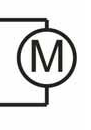
\includegraphics[scale=0.6]{DD.PNG}} & {\small{}Incrementa la potencia en la fase de balanceo, produciendo
mayor estabilidad y reduciendo el riesgo de caídas en el usuario\cite{Ossur}.} & {\small{}El mecanismo no es capaz de proveer trabajo positivo al amputado\cite{herr2014powered}.} & {\small{}Proprio Ossur $\circledR$}\tabularnewline
\hline 
{\small{}SEA}\footnote{SEA: Series Elastic Actuator /Actuador Elástico en serie.}{\small{}
\nomenclature[Series Elastic Actuator]{SEA}{\emph{Series Elastic Actuator} / Actuador Elástico en Serie}} & {\small{}\vspace{10 mm}}{\small \par}

{\small{}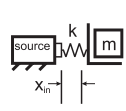
\includegraphics[scale=0.7]{SEAmodel.PNG}} & {\small{}Capaz de amplificar la potencia del actuador sobre una apropiada
longitud de zancada \cite{Paluska2006a}.} & {\small{}Soportan limitada salida de masa, poseen comportamientos
elásticos no lineales, limitaciones en la relación fuerza-velocidad,
limitaciones en la eficiencia del motor. Por otro lado, biológicamente
los músculos tienen alta eficiencia a bajas velocidades, mientras
que los motores eléctricos poseen alta eficiencia a altas velocidades\cite{Paluska2006a}.} & {\small{}-SPARKy (\emph{Spring Ankle with Regenerative Kinetics})\cite{Holgate2008,Bellman2008}.}{\small \par}

{\small{}-Prototipo transfemoral de la U. Vanderbilt \cite{Sup2008,Sup2009,Varol2010,Ha2011}.}\tabularnewline
\hline 
{\small{}CSEA}\footnote{CSEA: Cluthable Series Elastic Actuator / Actuador Elástico en Serie
con clutch}{\small{} } & {\small{}\vspace{15 mm}}{\small \par}

{\small{}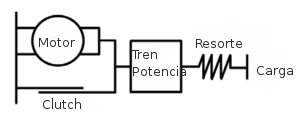
\includegraphics[scale=0.4]{CSEA.png}} & {\small{}Durante la fase de apoyo, el clutch es usado para almacenar
energía en la elasticidad del actuador. El primer prototipo requirió
de 1.8 J de energía eléctrica durante cada paso\cite{Rouse2014}.
A su vez, se comprobó una reducción energética externa del 70 \% en comparación
a los actuadores SEA\cite{Rouse2013}.} & {\small{}Este actuador tiene las mismas desventajas del SEA, la rigidez
invariable no permite entregar la máxima impedancia del actuador\cite{Rouse2014}.} & {\small{}Prototipo de rodilla de iWalk$\circledR$.}\tabularnewline
\hline 
{\small{}CV-SEA}\footnote{CVSEA: Continuosly Variable Series Elastic Actuator} & {\small{}\vspace{10 mm}}{\small \par}

{\small{}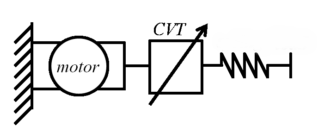
\includegraphics[scale=0.35]{CVSEA.PNG}}\footnote{{\small{}CVT: Continuosly Variable Transmission / Transmisión Continua
Variable.}} & {\small{}La transmisión de este actuador reduce el torque enviado
por el motor y permite su operación a altos niveles de eficiencia.
El CV-SEA optimiza el perfil de velocidad requerido durante la marcha,
reduciendo así las pérdidas\cite{Mooney}.} & {\small{}No se ha logrado implementar en prótesis de miembro inferior.} & \tabularnewline
\hline 
{\small{}SEAPS}\footnote{SEAPS: Series Elastic Actuator with Parallel Spring / SEA con Elasticidad
en Paralelo.} & {\small{}\vspace{5 mm}}{\small \par}

{\small{}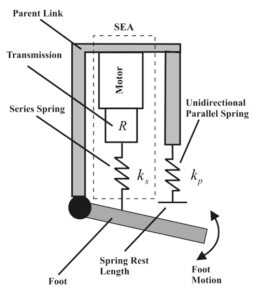
\includegraphics[scale=0.35]{BiOMmodel}} & {\small{}Tiene el potencial de variar el torque y la velocidad al
mismo tiempo \cite{Cherelle2014a}.} & {\small{}Las mencionadas anteriormente} & {\small{}Prótesis BiOM de iWalk $\circledR.$\cite{herr2011controlling,herr2014powered,han2012controlling,han2014controlling}}\tabularnewline
\hline 
{\small{}SEDA}\footnote{SEDA:Series Elastic Damper Actuator /Actuador Elástico con Amortiguador
en serie.} & {\small{}\vspace{5 mm}}{\small \par}

{\small{}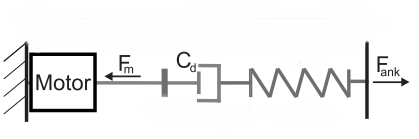
\includegraphics[scale=0.3]{SEDA.PNG}} & {\small{}Requiere el menor pico de potencia en la intención de descenso
de escalones\cite{Eslamy2013}.} & {\small{}Para otras intenciones de marcha no se ha encontrado el beneficio.\cite{Eslamy2013}} & {\small{}No implementado a la fecha.}\tabularnewline
\hline 
{\small{}PEDA}\footnote{PEDA: Parallel Elastic Damper Actuator / Actuador Elástico con Amortiguador
en paralelo.} & {\small{}\vspace{5 mm}}{\small \par}

{\small{}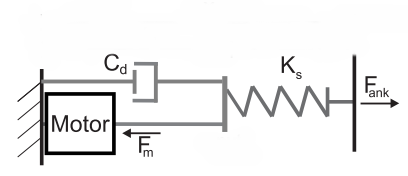
\includegraphics[scale=0.3]{PEDA.PNG}} & {\small{}Se encontró que el motor requiere menos fuerza en comparación
al SEA en el inicio de la fase de apoyo.\cite{Eslamy2013}} & {\small{}Incrementan los requerimientos energéticos al final de la
misma fase.\cite{Eslamy2013}} & {\small{}No implementado a la fecha.}\tabularnewline
\hline 
EEA\footnote{EEA: Explosive Elastic Actuator / Actuador Explosivo Elástico} & {\small{}\vspace{5 mm}}{\small \par}

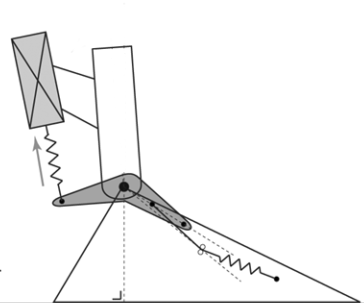
\includegraphics[scale=0.25]{EEA} & {\small{}Utiliza el principio de la distribución óptima de potencia
\cite{Wahl2013}. Genera hasta 3.3 W/kg de potencia pico con un requerimiento
de 60 W eléctricos.}{\small \par}

Actua durante toda la fase de apoyo \cite{Cherelle2014b}. & {\small{}Existen variaciones cinemáticas en el tobillo. No es antropométrica
\cite{Cherelle2014}.} & AMP-foot 2.0 {\small{}\cite{Cherelle2014} y 2.1 }\cite{Cherelle2014b}.\tabularnewline
\hline 
{\small{}VSA}\footnote{VSA: Variable Stiffness Actuator) / Actuador de Elasticidad Variable.} & {\small{}\vspace{10 mm}}{\small \par}

{\small{}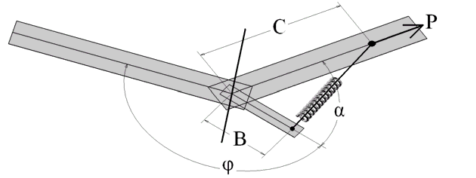
\includegraphics[scale=0.25]{maccepa2.PNG}} & {\small{}Mecanismo robótico capaz de cambiar la rigidez de la articulación
a través del tensionamiento de un resorte. Puede proveer hasta el
100 \% de la potencia en la propulsión. \cite{Cherelle2014a}} & {\small{}Requiere de dos motores para controlar la variable elástica,
por lo que requiere mayor energía que los SEA.\cite{Geeroms2013}Es
un sistema más pesado, y es mucho más complejo que el SEA. \cite{Cherelle2014a}} & {\small{}CYBERLEG project (Prototipo)}\tabularnewline
\hline 
\end{longtable}
\par\end{center}


\section*{\label{sec:Ap=0000E9ndice-A}Apéndice C: Antecedentes del autor y del grupo de investigación en temas afines.}


\subsubsection*{Trabajos de grado y publicaciones:}
\begin{itemize}
\item Prieto-Parrado, E. (2014).``\emph{Diseño, simulación y obtención
de un prototipo de pie de alto impacto para amputados de miembro inferior}''
(Tesis de maestría meritoria). Universidad Militar Nueva Granada,
Bogotá. 


En este trabajo se tomaron los parámetros antropométricos de una determinada
población colombiana para adaptarlos al diseño de una prótesis de
alto rendimiento para amputados de miembro inferior. Se realizaron
pruebas experimentales con diferentes composiciones de hojas laminadas
de fibra de carbono para hallar la mejor relación esfuerzo-rigidez
del material y posteriormente se verificó el diseño con la técnica
de simulación en elementos finitos (FEA) para finalmente llevarlo
a su construcción. 

\item Prieto-Parrado, E. y Cortés-Rodríguez, C. (2016). \emph{``Estado
actual y problemática en prótesis de miembro inferior: revisión''.
}En revisión por parte de la revista Ingeniería Biomédica ISSN No.1909-9991.

\end{itemize}

\subsubsection*{Eventos}
\begin{itemize}
\item Ponente en el Solidworks world 2013 en Orlando, Florida - Walt Disney
World Swan and Dolphin Resort. Proyecto expuesto: Prótesis de miembro inferior (Rodilla).
\end{itemize}

\subsubsection*{Experiencia en Investigación y desarrollo:}

Coordinador de proyectos en I+D para la Industria Militar de Colombia
(2009-2014): Dirección, coordinación, seguimiento, valoración tecnológica,
propiedad industrial, gestión administrativa y técnica de proyectos
en investigación y desarrollo tecnológico enfocados al sector defensa,
entre los proyectos más destacados relacionados a la temática de la
propuesta se encuentran:
\begin{enumerate}
\item Reingeniería a prótesis de rodilla hidráulica policéntrica. Asociados:
Universidad Militar Nueva Granada (UMNG) - Grupo DAVINCI y Hospital
Militar Central (HMC). Entregables:

\begin{itemize}
\item Documento preclínico para inicio de ensayos en paciente con la prótesis desarrollada.
\item Validación del prototipo mediante máquina de ensayos protésicos de acuerdo a ISO 10328.
\item Prototipo de rodilla hidráulica policéntrica.
\end{itemize}
\item Reingeniería a prótesis de pie. Asociados: UMNG-DAVINCI y Hospital
Militar Central (HMC). Entregables: 

\begin{itemize}
\item Documento preclínico para inicio de ensayos en paciente con la prótesis desarrollada.
\item Validación según norma ISO 22675 del prototipo mediante máquina de ensayos.
\item Prototipo de pie protésico de bajo perfil.
\end{itemize}

\end{enumerate}

\subsubsection*{Antecedentes (en la temática) del Grupo de investigación GIBM-UNCB}
\begin{itemize}
\item Rosas-Rosas, X. (2015). Análisis biomecánico para prescripción ortésica
en postoperatorio de cirugía multinivel para diplejia espástica. Estudio
de caso, \emph{Tesis de maestría}. Universidad Nacional de Colombia,
Bogotá.
\item Silva-Castellanos, C. (2015). Modelamiento De La Marcha Humana Con
Prótesis De Miembro Inferior Mediante Herramientas De Simulación Dinámica
(“ Una Aplicación en Opensim”). \emph{Tesis de maestría}. Universidad
Nacional de Colombia, Bogotá.
\item Rodríguez-Montaño, O.L. (2015). Modelación de órtesis personalizadas
para alivio de presiones plantares en pie diabético. \emph{Tesis de
maestría}. Universidad Nacional de Colombia, Bogotá.
\item Rodríguez-Montaño O.L., Cortés-Rodríguez C.J., and Silva-Caicedo O. Finite element model of the foot to estimate center of pressure trajectory. Proceedings of the 14th international Symposium on Computer Simulation in Biomechanics. 01-03 August 2013. Pontanegra, Natal, Brazil.
\item C. J. Cortes-Rodriguez, O. L. Rodríguez-Montaño, O. Silva-Caicedo. Mathematisches Modell auf Grundlage von dynamischer Pedobarographie und FEM fur Erzeugung der Oberflächentopographie in der Fuß-Schuh-Schnittstelle fur Entlastung des plantaren Drucks. 9. Jahrestagung der Deutschen Gesellschaft fur Biomechanik (DGfB). 6.-8. Mai 2015. Bonn. Germany.
\item Oscar Libardo Rodríguez-Montaño, Carlos Julio Cortés-Rodríguez, Octavio Silva-Caicedo. Modeling and computational comparison of foot orthosis for plantar pressure relief. XXV Congress of the International Society of Biomechanics. July 12th  16th 2015, Glasgow, UK.
\item David L. Maldonado Guzman, Carlos Julio Cortes Rodriguez. Approximation to the mathematical modeling of articular contact by applying the differential geometry /kinematic (dg/k) method. XXV Congress of the International Society of Biomechanics. July 12th  16th 2015, Glasgow, UK.
\end{itemize}
\end{document}
